%
% Copyright (c) 1996 Bunyip Information Systems Inc.
% All rights reserved
%
% Archie 3.5
% August 1996
\documentclass[10pt,oneside]{book}

\usepackage{fullpage}
\usepackage{epsfig}
\usepackage{longtable}

%\addtolength{\oddsidemargin}{72pt}
%\addtolength{\textwidth}{-72pt}

%
%  Do not want any indentation of the paragraphs !!!
%
\setlength{\parindent}{0pt}



\begin{document}

%
% Defs
%

\def\HUGE{\@setsize\HUGE{40pt}\xxvpt\@xxvpt}


\newcommand{\Chapter}[1]{\hspace{-72pt}\chapter{#1}}


\newcommand{\version}{3.5}

\newcommand{\marginnew}[1]{
  \marginpar[\hfill\begin{minipage}{#1}
  \epsfig{file=figs/new.eps,width=#1} \end{minipage}]
  {\begin{minipage}{#1}
  \epsfig{file=figs/new.eps,width=#1}
  \end{minipage}}}

\newlength{\marginwidthhalf}
\setlength{\marginwidthhalf}{\marginparwidth}
\divide \marginwidthhalf by 2
\newcommand{\new}{
 \addtocontents{toc}{\protect\marginnew{\marginwidthhalf}}
  \marginnew{\marginparwidth}}
\newcommand{\New}{\marginnew{\marginparwidth}}


\newcommand{\NOTE}{\marginpar[\hfill\begin{minipage}{\marginparwidth}
  \epsfig{file=figs/note.eps} \end{minipage}]{\begin{minipage}{\marginparwidth}
  \epsfig{file=figs/note.eps} \end{minipage}}}


%
%
%

\newlength{\alertboxwidth}
\setlength{\alertboxwidth}{\textwidth}
\addtolength{\alertboxwidth}{-10pt}

\newcommand{\alertbox}[1]{\vspace{0.1in}\noindent\framebox{\parbox{\alertboxwidth}{#1}}\vspace{0.1in}}


\newcommand{\BUGBUG}[1]{\vspace{0.1in}\noindent\framebox{\framebox{\parbox{\alertboxwidth}{#1}}}\vspace{0.1in}}



\setlength{\parskip}{5pt}


\newcommand{\param}[1]{\hspace{0.5in}\texttt{#1}}
\newcommand{\Param}[1]{\texttt{#1}}

\newcommand{\comm}[1]{\param{\% #1}}
\newcommand{\Comm}[1]{\Param{\% #1}}

\newcommand{\path}[1]{\param{#1}}
\newcommand{\Path}[1]{\Param{#1}}

\newcommand{\archie}{\symbol{126}archie}
\newcommand{\Archie}{<archie home>}

\newenvironment{TTentry}[1]
 {\begin{list}{}{\renewcommand{\makelabel}[1]{\texttt{##1:}\hfil}%
   \settowidth{\labelwidth}{\texttt{#1:}}%
   \setlength{\leftmargin}{\labelwidth}
   \addtolength{\leftmargin}{\labelsep}
 }}%
 {\end{list}}



%
%  FAQ Question and Answers defs
%

\newcommand{\Question}[1]{\noindent\textbf{#1}}
\newcommand{\Answer}[1]{\begin{quote} #1 \end{quote}}



%
%
%
%
%

\newcounter{SidePrintX}
\setcounter{SidePrintX}{468}

\newcounter{SidePrintY}
\setcounter{SidePrintY}{144}


\newcommand{\SidePrint}[7] {
  \special{
    ! userdict begin
        /CurrentPage 0 def
        /bop-hook{
          /CurrentPage CurrentPage 1 add def
          CurrentPage 1 le
          { gsave 200 80 translate 90 rotate
            /Times-Roman findfont
            #2 scalefont setfont
            0 0 moveto
            #3 setgray
           (#1) show
            1 setlinewidth
            0 -5 moveto #4 setgray (#1) stringwidth rlineto stroke
            /Times-Roman findfont
            #6 scalefont setfont
            0 #6 neg moveto #7 setgray (#5) show
            grestore
          } if
        } def
        end
     }
  }


%            10 setlinewidth
%            0 0 moveto 0 setgray (#1) stringwidth rlineto stroke

%
% Title Page
%



%
% Copyright (c) 1996 Bunyip Information Systems Inc.
% All rights reserved
%
% Archie 3.5
% August 1996
%
% Title page
%



%\title{ Archie \\ Version \version \\ System Manual}

%\author{ Bunyip Information Systems}


%\maketitle


\begin{titlepage}


\SidePrint{Archie 3.5}{144}{0.87}{0}{System Manual}{36}{0.80}

\vspace*{\fill}

\hfill{\Large Bunyip Information Systems, Inc.} 

\end{titlepage}

\newpage

\thispagestyle{empty}
\vspace*{\fill}

\small{
\noindent Bunyip Information Systems Inc. \\
310 Ste. Catherine St. W \\
Suite 300 \\
Montreal, Quebec \\
Canada H2X 2A1 \\

\begin{tabbing}
Tel: \hspace*{5pt}\=(514) 875-8611 \\
Fax: 	            \>(514) 875-8134 \\
\end{tabbing}


\begin{tabbing}
email: \= info@bunyip.com \\
       \>	archie-group@bunyip.com \\
	     \> archie-admin@bunyip.com \\
\end{tabbing}


\noindent
Archie is a registered trademark of Bunyip Information Systems Inc., Canada,
1990.\\
Copyright  1993, 1994, 1995, 1996 by Bunyip Information Systems Inc.
No part of this manual may be reproduced, stored in a retrieval system, or
transmitted, in any form or by any means, electronic, mechanical,
photocopying, recording, or otherwise, without the prior written permission
of Bunyip Information Systems. \\
This product includes software developed by the University of California,
Berkeley and its contributors.
}




%
% table of contents
%

\newpage
\pagenumbering{roman}
\setcounter{page}{1}
\tableofcontents



%
% Body of text
%

%
% Copyright (c) 1996 Bunyip Information Systems Inc.
% All rights reserved
%
% Archie 3.5
% August 1996
%
% intro.tex
%

\chapter{Introduction}

\pagenumbering{arabic}
\setcounter{page}{1}


It was inevitable that the technology under which Archie was built changed.
With the introduction of faster applications and newer media on the Internet,
Archie had to reshape its structure to accomodate these new factors and
stay in the race.

Speed in this day and age is a big gain and Archie is thought to have
achieved it with the utilization of a string indexing tree for faster string
searches.

As for the World Wide Web and its many new faces, Archie also introduces its
latest web crawling and indexing engine.  In addition, a new web interface has
been added to accomodate the web users.  And with a few more newly added
features and face-lifts, Archie v3.5 is ready to undergo deployment.

This manual is an attempt to clarify the many components of Archie v3.5 and
its functionality.  Please keep in mind that this manual is also undergoing
changes, so we appreciate any comments sent to archie-group@bunyip.com.

What follows is the list of added features in Archie v3.5. You will find in
the table of contents, symbols such as the one in the margin, to help you
find the relevant documentation concerning the new features. \New

\begin{itemize}
\item Support for a new database module (webindex):
  \begin{itemize}
    \item Retrieval of HTML pages through HTTP protocol.
    \item Keyword extraction.
    \item Controlled crawling of the WWW.
    \item Site by site basis.
    \item Content extraction.
    \item Configurable stoplist (keyword exclusion).
  \end{itemize}
\item New database structure:
  \begin{itemize}
    \item A more reliable and independent database structure. 
  \end{itemize}
\item New strings search engine:
  \begin{itemize}
    \item Based on a paged, tree structured strings index.
    \item Faster searches.
    \item Less memory required.
    \item More disk space needed for construction of the index.
  \end{itemize}
\item New search interface:
  \begin{itemize}
    \item New WWW (CGI compliant) front-end to the Archie database.
  \end{itemize}
\item A better domain filter for any database:
  \begin{itemize}
    \item Results can be pre-configured to return in a certain order (e.g. FTP sites closest to the server first).
    \item Configurable on a server basis.
  \end{itemize}
\item General new features:
  \begin{itemize}
    \item Support for ls-lR.gz files.
    \item ISO-Latin-1 support for searches.
  \end{itemize}
\end{itemize}



\section{Future}

We hope in the very near future to be able to produce
the following list of features. If you have any suggestions
to add to the list please feel free to contact us at
archie-group@bunyip.com:

\begin{itemize}
  \item  Search tools:
    \begin{itemize}
      \item Add boolean searches.
      \item Allow other types of searches. (For example, return a
            list of hosts in any database and when they were last updated.)
      \item Multi-lingual Web front-end.
    \end{itemize}
  \item  Database:
    \begin{itemize}
      \item  An automated check-up program that runs periodically on the
             databases.  It will check the consistency of the database and
             fix any errors it runs into.   This will reduce the amount of
             time an Archie administrator needs to spend maintaining an Archie server.
      \item  Improve on filters and parsers to handle strange and unusual site
             listings.
      \item  Parallelize the parsing and updating of different databases.
      \item  Build multiple databses with the same access method.
    \end{itemize}
  \item  Management tools:
    \begin{itemize}
      \item  CGI web interface to allow web and FTP administrators to register
             their sites automatically.
      \item  Replace ``host\_manage'' with a new method for managing the
             host\_db database.
      \item  Statistical tools.
    \end{itemize}
\end{itemize}


% If you somehow got this file without fullpage.sty,  delete
% ``fullpage'' from the list of style options.  It just pulls out the
% margins a bit.
\documentstyle[11pt,twoside,fullpage]{article}
% New commands
%-------------
% Intro copied from prospero-protocol-v5.txt

% for meta-symbols
\newcommand{\meta}[1]{{\bf \mbox{\(<\)#1\(>\)}}}
% for literal tokens.
\newcommand{\lit}[1]{{\tt \mbox{#1}}}
%for attributes
\newcommand{\atr}[1]{\mbox{\sc #1}}
% for identifying text
\newcommand{\text}[1]{{\em #1}\/}

% Start and end of One or More
\newcommand{\ooms}{\([\,\)}
\newcommand{\oome}{\(\,]^+\)}
% start and end of zero or more
\newcommand{\zoms}{\([\,\)}
\newcommand{\zome}{\(\,]^*\)}
% Start and end of zero or one
\newcommand{\zoos}{\([\,\)}
\newcommand{\zooe}{\(\,]\)}
% start an OR
\newcommand{\ors}{{\bf (\,}}
\newcommand{\ore}{{\bf \,) }}
\newcommand{\metaor}{{\em \,or\, }}
\newcommand{\hexnum}[1]{\(\mbox{#1}_{16}\)}
\newcommand{\unix}{{\sc unix}}
\newenvironment{command}{\begin{verse}\sloppy}{\end{verse}}
\newcommand{\commandsize}{\large}

%\newtheorem{example}{Example}
% Uncomment this for almost-double spacing
%\renewcommand{\baselinestretch}{1.7}
%\newcommand{\hozline}{\rule{\textwidth}{0.3mm}}
%\newcommand{\hozline}{\makebox[\textwidth]{\hrulefill}}
%\newcommand{\bex}{\begin{example} \begin{rm}}
%\newcommand{\eex}{$\Box$ \end{rm} \end{example}}
%\newcommand{\cbs}{\chgbarbegin}
%\newcommand{\cbe}{\chgbarend}
%\newcommand{\cbs}{}
%\newcommand{\cbe}{}

%\newcommand{\ptag}{\begin{flushright} {\rm ($P$)} \end{flushright} }


\begin{document}

\pagenumbering{arabic}
\pagestyle{plain}

\renewcommand{\thepage}{\arabic{page}}


\begin{titlepage}

\renewcommand{\thefootnote}{}
\footnotetext{\hspace*{-21pt}
Digital copies of the latest revision of this document may be obtained
through Prospero as
\mbox{\verb"/papers/subjects/operating-systems/prospero/doc/user-manual.PS.Z"},
in the \mbox{\tt \#/INET/EDU/ISI/swa} virtual system, or through
Anonymous FTP from \mbox{\tt PROSPERO.ISI.EDU} as
\mbox{\verb"/pub/prospero/doc/prospero-user-manual.PS.Z"}
}
\footnotetext{\hspace*{-21pt}
This work was supported in part by the National Science
Foundation (Grant No. CCR-8619663), the Washington Technology Center,
Digital Equipment Corporation, and the Defense Advance Research
Projects Agency under NASA Cooperative Agreement NCC-2-539.
The views and conclusions contained in
this document are those of the authors and should not be interpreted as
representing the official policies, either expressed or implied, of
any of the funding agencies.
The authors may be reached
at USC/ISI, 4676 Admiralty Way, Marina del Rey, California\ \ 90292-6695, USA.
Telephone +1 (310) 822-1511, email \mbox{\verb"info-prospero@isi.edu"}.  }
\renewcommand{\thefootnote}{\arabic{footnote}}


\vspace*{\fill}
\begin{center}
\LARGE Prospero User's Manual\\
\Large Version 5\\
\vskip 1.5em
{\large Draft of 8 July 1993} \\
{\large Document Revision No. 0.2} \\
\end{center}
\vspace{.5in}

\Large \hspace*{\fill} B. Clifford Neuman
%\footnotetext{\hspace*{-18pt}
%	To Contact the Authors: \\
%	Electronic Mail: \mbox{\verb"info-prospero@isi.edu"} \\
%    Telephone: +1 (310) 822-1511 \\
%    Mail: USC Information Sciences Institute, 4676 Admiralty Way,
%  Marina del Rey, California  90292--6695\ \ U.S.A.
%}
\hfill Steven Seger Augart \hspace*{\fill} \\
\vspace{.2in}
\begin{center}
\Large Information Sciences Institute \\
University of Southern California
\end{center}
\vspace*{1.2in}
\vspace*{\fill}
\end{titlepage}

\tableofcontents

\section{Introduction}

The Prospero file system is based on the Virtual System Model.
\nocite{nfclosure,vsmldos}
% \nocite{phdneuman,vsmtp}
It differs from traditional distributed file systems in several ways.
In traditional file systems, the mapping of names to files is the same
for all users.  Prospero supports user centered naming: users
construct customized views of the files that are accessible.  A
virtual system defines this view and controls the mapping from names
to files.  Objects may be organized in multiple ways and the same
object may appear in different virtual systems, or even with multiple
names in the same virtual system.

Prospero directories can contain references to files and directories
that are stored on remote nodes.  This allows distribution at a much
finer level of granularity than is possible in traditional distributed
file systems.  Prospero also provides several tools to support
customization.  Among them are the union link and the filter.

\section{The Directory Mechanism}

{In \samepage Prospero, the global file system consists of a collection of {\it
virtual file systems}.  Virtual file systems usually start as a copy
of a prototype.  The root contains links to files or
directories\footnote{To distinguish them from directories and links in
traditional systems, and because they are often illusory, directories
and links in Prospero are sometimes referred to as virtual directories and
virtual links.} selected by the user.  Directory links can be of
several types: conventional, union, and filtered.}

A conventional link is similar to a hard link in traditional file
systems.  It may be made to any type of object, including a directory.
It maps a name for an object to the information needed to access the
object.  As long as an unexpired link to an object exists the object
may be accessed by that name.  If the object moves, a forwarding
pointer will allow continued access using the same name.  An object is
only deleted when no unexpired links to it remain.

A union link can only be made to a directory.  With a union link, the
objects included in the linked directory become part of the virtual
directory containing the link.  Thus, the contents of a virtual
directory are the union of the collection of conventional links it
contains, and the contents of all directories included through union
links.

Filters may be attached to either type of link.  A filter alters the
set of links that are seen in directories whose paths pass through the
filtered link.  A filter can specify which links are to appear and
which are to be ignored, it can change the features of individual
links, or it can synthesize new links that are not in the original
directory.  Client-side filters are written in C and are dynamically
linked during name resolution.  A filtered link contains a reference
to the filter and any arguments required by the filter.

\section{Using the Prospero File System}

This section assumes that Prospero has already been installed on your
system.  Section~\ref{new_system} describes the installation
procedure.

To use Prospero you must first determine the name of the directory
that contains the executables.\footnote{By default, the installation
directory is {\it /usr/pfs/bin}.} 
\begin{itemize}
\item{CSH users}  That directory
contains a file called vfsetup.source, the contents of which must be
read by the shell.  This can be accomplished by {\tt source}ing it.
For example, if the Prospero file system binaries are stored in {\it
/usr/pfs/bin} you should either execute the following command or add
it to your {\it .cshrc} file:

\begin{verbatim}
    source /usr/pfs/bin/vfsetup.source
\end{verbatim}

\item{SH users}  That directory
contains a file called {\tt vfsetup.profil}, the contents of which must be
read by the shell.  This can be accomplished with the {\tt .} command.
For example, if the Prospero file system binaries are stored in {\it
/usr/pfs/bin} you should either execute the following command or add
it to your {\it .profile} file:

\begin{verbatim}
    . /usr/pfs/bin/vfsetup.profil
\end{verbatim}

\end{itemize}

Before you can begin using the Prospero file system a virtual system
must be created for you.  Section~\ref{creating_vfs} explains how the Prospero
site administrator can create a new virtual system.   Don't be frightened away from
experimenting by these comments!    Most Prospero
sites support a {\it guest} virtual system which can be used until your
own virtual system is created.   Prospero, as shipped, is configured
so that once you compile the clients you can type ``{\tt vfsetup
guest}'' and start working right out of the box using a guest virtual
system at the USC Information Sciences Institute.

To use a virtual system, you must first execute the {\tt vfsetup}
command to initialize your environment.  For example, if the name of
your virtual system is {\it guest} you should execute the following
command:

\begin{verbatim}
    vfsetup guest
\end{verbatim}

\section{Using the menu browser}

The menu browser provides a simple straightforward interface to the
Prospero file system.   

\subsection{Starting it up}
In the simplest case, invoke it as ``{\tt menu}''.  If you are vfsetup to a
virtual system and there is a directory named {\tt /MENU} in that virtual
system, it will use that directory.  If you have not run the  {\tt
vfsetup} command or if there is no link named {\tt /MENU} in the
current virtual system, it will bring up the default menu for your
site.  We have set up a default menu for people who compile Prospero
to use the default site, the ISI guest site.

If you are already vfsetup to a virtual system, you can invoke the
menu browser as ``{\tt menu {\it linkname}}''.  The browser will
display the Prospero directory {\it linkname} as its root menu.

\subsection{Using it}

The browser will display a numbered list showing the contents of the
directory.  The items in the list will be followed by one of four
characters:

\begin{itemize}

\item[{\tt .}]  A file.  If it is a data file, you will be able to retrieve
it and save it.  If it is a text file, you can retrieve it and view
it, and then have the option of mailing it, saving it, or printing it.

\item[{\tt $>$}] A directory (submenu).  You can select it to see the
contents, and then type {\tt u} to go up to the previous menu.

\item[{\tt \verb"]"}]  A portal.  This represents a service you will have to
connect to via {\em telnet} or some similar protocol.  Select it in
order to receive some instructions and begin a {\em telnet} session.

\item[{\tt :}] A search.   It will display some initiali documentation.  It may
ask you to select among several possible searches, and will then
prompt you for what you are searching for.  Later versions of the menu
browser will check what you type at the prompts to make sure the
format is correct.  Type {\tt ?} at the
beginning of any line in order to receive further documentation  about
the meaning of that line.\footnote{If you want to search for an item
beginning with a literal {\tt ?}, then precede it with a backslash to
escape it. %type {\tt \verb"\"?}}.
If you want to search for something beginning with a backslash, then precede it with
another backslash to excape it.
%beginning with a literal \verb"\", then type \verb"\\".
}

The results of the search will be displayed as a new menu that
contains a list of the items that matched the search, possibly
including subdirectories.\footnote{N.B.: If you make a search that is relayed
through the Prospero/Gopher gateway, you may be immediately presented with a
submenu containing a single item, and will have to open that item to
see the results of your search.}
\end{itemize}

Type the number of the item you wish to explore in order to explore
that item.  Type {\tt q} to quit.

\subsection{Making your own menus}

The main current deficiency of the menu browser interface is that at
the moment the browser is read-only.  For now, you will have to learn
a bit about the command-line client interface in order to set up new
directories under Prospero, in order to change the names of menu
items, and in order to create new links.  We are currently working to
put most of the power of the command line interface into the menu
browser so that one does not have to use two user interfaces for most
purposes. 

To make your own menus, you will have to learn the {\tt set\_atr}
command, to set attributes on objects, the {\tt vln} command, to make
new links, and the {\tt vmkdir} command, to make subdirectories.

\section{Using the command-line clients}

\subsection{File Names}

The slash, colon, pound sign, open and close parenthesis, and backslash
({\tt /, :, \#, (, ),} and \verb"\") are special characters in
Prospero.  The slash separates components of file names and the colon
separates information identifying a virtual system from the name of a
file within the virtual system.  These characters should not appear in
any component of a file name unless they have been quoted.

All special characters, including the backslash, can be quoted by
preceding them with a backslash.  This is important to know,
especially when you're working with names returned by the Prospero
GOPHER-GW gateway; those names often contain colons, slashes, and other special
symbols.

The slash is used in user-level names to indicate moving into a
subdirectory, just as it does in {\sc unix}-like operating systems.
This is the only important special character to know about upon the
first reading of this document; the others are more specialized.

By default, names are resolved relative to the active virtual system.
If a colon ({\tt :}) appears in a name, the name is resolved relative
to the name space identified preceding the colon.  If the character
preceding the colon is a pound sign ({\tt \#}), then the name
preceding the pound sign will be treated as an alias for a previously
specified virtual system.  For this reason, virtual systems should not
have names ending in a pound sign.  A double colon ({\tt ::}) is the
closure operator.  When encountered, the name space identified by the
{\sc closure} attribute\footnote{See the Attributes appendix to the Prospero
Protocol specification for the definition of this attribute} of the
object named before the double colon is used to resolve the name that
follows.

The pound sign ({\tt \#}) is also used to resolve name conflicts when
the same component of a name is used by more than one object.  In this
case the pound sign is followed by the magic number of the desired
object.  For this reason, unless quoted, the pound sign should not be
used in a component of a file name if followed by a number (including
sign), and if there are no intervening non-numeric characters between
the pound sign and the end of the component.

The pound sign ({\tt \#}) is additionally used to indicate that a
particular named union link is to be followed when resolving a name,
or to indicate that a filter is to be applied.  In these cases, the
pound sign is the first character of a component in a name and it is
followed by the name of the union link to be followed or the name of
the filter to be applied.  For this reason, unless quoted, the pound
sign should not be used as the first character in a component of a
file name (unless the full name of the component is {\tt \#}).  

The open and close parenthesis ({\tt (} and {\tt )}) are used to
delimit the arguments to a filter specified as part of a file name.
The arguments immediately follow the name of the filter (which itself
follows a single or double pound sign).  If the filter name follows a
single pound sign, it is a client-side filter.  If the filter name
follows a double pound sign, it is a server-side filter.  

Therefore, it follows that if the name of a union link ends in a {\tt
)}, and it is explicitly specified as part of path name, the {\tt )}
must be quoted.

We have not yet specified a syntax for
differentiating between client-side pre-expansion and post-expansion
filters, nor for differentiating among directory, hierarchy, object,
update, and link filters.


If no arguments are required, the null argument list {\tt ()} must be
included.  These uses of the \# convention to specify a filter is not
currently supported.

\paragraph{Loadable Filters}

The above filter syntax works for predefined filters.  Loadable
filters are not currently used.  The working definition of their
syntax, which is being redefined due to it being difficult to parse,
is: If the filter name contains an unquoted colon or slash, then it is
interpreted as a loadable filter.  If the filter name does not, it is
interpreted as a predefined filter.  Note that you can specify a
loadable filter in the current virtual directory by prefixing its name
with the sequence {\tt ./}.


\subsection{Finding Things}

The Prospero file system provides tools that make it easier to keep
track of and organize information in large systems.  When first
created, your virtual file system is likely to contain links to
directories that organize information in different ways.  As the
master copy of each of these directories is updated, you will see the
changes.  You may customize these directories.  The changes you make
to a customized directory are only seen from within your own virtual
system, but changes made to the master copy will also be visible to
you.  See section~\ref{customizing} for instructions on customizing a
directory.

Users are encouraged to organize their own projects and papers in a
manner that will allow them to be easily added to the master
directory.  For example, users should consider creating a virtual
directory that contains pointers to copies of each of the papers that
they want made available to the outside world.  This virtual directory
may appear anywhere in the user's virtual system.  Once set up, a link
may be added to the master author directory.  In this manner, others
will be able to find this directory.  Once added to the master
directory, any future changes will be immediately available to other
users.

To add a link to the master copy of any of the shared directories,
send a message to your site administrator.  The address should be {\it
pfs-administrator} on the primary system for the site.  If you are
using a virtual system stored at the USC Information Sciences Institute, the
address would be {\it pfs-administrator@isi.edu}.

\subsection{The Commands}

This section 
%steps though the process of creating and using a virtual file system.
%It  
assumes that the Prospero file system has been installed on the system
being used.  Later sections explain how to install the Prospero file
system at a new site and on individual systems.

Most of the commands that are specific to the Prospero file system
take a debug option.  The form is {\em -D\#} where \# is an optional
integer and specifies the level of detail.  The higher the integer,
the greater the detail.  By itself, {\em -D} sets the debugging level
to 1.  Debugging levels of 9 and above display the actual Prospero
protocol messages that go across the network.  

\subsubsection{Initialization and Changing Virtual Systems}

\begin{verbatim}
    vfsetup [-n host path , [-r,v] name , -f file]
\end{verbatim}

The {\tt vfsetup}\footnote{Because it changes environment variables,
this command only has an affect when its output is read by the shell.
If {\it vfsetup.source} has been {\tt source}ed, then {\tt vfsetup} is
an alias which will call the {\it vfsetup} executable in the
appropriate manner.} command sets up the selected virtual system.  It
adds the appropriate directories to the search path and sets all
necessary environment variables. {\tt vfsetup} can be called in
several ways.  With no arguments, it reads the file {\it
\verb+~+/.virt-sys} and uses the information found to access the
virtual system description.  The {\em -v} option takes the name of the
virtual directory containing the system description.  The {\em -n}
option takes the name of a host and the physical name of the virtual
directory on that host that contains the virtual system description.
The {\em -f} option takes the name of a Unix file that is to be read
in place of {\it \verb+~+/.virt-sys}.

It is also possible to set up a virtual system by specifying its name.
If the {\em -r} option is specified, the name is taken to be the
default name for the virtual system at the local site.  If the name is
specified without a modifier, the name is looked up in the {\sc
/virtual-systems} directory of the presently active virtual system
(the site default is used if no virtual system is presently active).
For example, if the name of your virtual system is {\it guest} you can
set up the virtual system using following command.

\begin{verbatim}
    vfsetup guest
\end{verbatim}


\subsubsection{Creating Directories}

\begin{verbatim}
    vmkdir directory
\end{verbatim}

{\tt vmkdir} creates a virtual directory with the selected name and
adds a link from its parent directory.

\subsubsection{Adding and Deleting Links}

\paragraph{vln}

\begin{verbatim}
    vln [-i, -u, -s, -m, -a] {-e access-method-info, -n host hsoname, linkname } newname
\end{verbatim}

{\tt vln} adds a new link to a directory.  {\em oldname} is an
existing name for the object to which the link is to be made.  {\em
newname} is the name of the new link.  The {\em -u} option indicates
that the new link is to be a union link.  The {\em -s} option is used
to specify a symbolic link.  The {\em -i} option is used to specify an
invisible link which will not be displayed in a normal directory listing.

The {\em -n} option (short for {\em native})  requires the specification of the
name of the host containing the target.  The {\em -n} option indicates
that the native information for the target has been specified.  {\em
host} is the name of the host on which the target resides and {\em
oldname} is the name of the target on that host.  If the {\em -s}
option has also been specified, then {\em host} is the name of the
virtual system to which oldname is relative.

The {\em -e access-method-info} (external) option indicates that the
object resides on a host that does not run Prospero.  There are are
number of possible values for the {\em access-method-info}:
\begin{description}
\item[GOPHER {\em host}({\em port}) {\em gopher-selector} \{BINARY {\em or} TEXT\}]
This access method indicates that the object can be retrieved by
sending the selector string {\em gopher-selector} to a server running
at port {\em port} on host {\em host}.  You must specify whether you
want the object to be retrieved using the Gopher binary or text
retrieval methods.
\item[TELNET {\em host}[({\em optional-port})] {\em introductory-message}]
If you do not provide a port inside parentheses, then the default {\em
telnet} port will be used.  The {\em introductory-message} will be
displayed before the user connects to the service.  For example:
\begin{quote}
Type {\tt LAX} at the prompt in order to get the current Los Angeles weather
forecast; type {\tt X} to quit.
\end{quote}
\item[AFTP {\em host} {\em path} \{BINARY {\em or} TEXT\}]  This access method
specifies that the object can be retrieved via anonymous FTP, using
either the {\em binary} or {\em text} retrieval methods.
\item[AFS {\em afs-path}]  This access method specifies that the object is
available through the Andrew File System.  Its name via {\sc afs} is {\em
afs-path}.  You should not precede the {\em afs-path} with {\tt
/nfs/afs}, {\tt /afs}, or whatever the prefix is that your local
system prepends to {\sc afs} names.
\item[{\em \#-of-access-method-args} {\em method-name} \\
{\em host-type} {\em host} {\em hsoname-type} {\em hsoname} {\em any additional args}]
This type is used to provide an explicit value for the {\sc access-method}
attribute.  See appendix A of the Prospero protocol specification for
a discussion of the format of this attribute.  

\end{description}

Note that some of the host names specified in these access methods may
include a port number inside parentheses.  You will probably have to
quote the port number so that whatever shell you use does not
interpret it in a way you don't expect.

\subparagraph{Some examples of making links}

Here I'm making an external Gopher TEXT link to a recipie:
\begin{verbatim}
vln -e GOPHER 'ashpool.micro.umn.edu(70)' 0/fun/Recipes/Balls/rum-balls TEXT rum-balls
\end{verbatim}
I can now retrieve this document with {\tt vget} or by running ``{\tt
menu .}''.

Here I'm making a link to a telnettable service.  In this case, I have
decided to make the {\em introductory-message} a null string, since
the service I'm linking to has its own excellent documentation facilities:
\begin{verbatim}
vln -e TELNET 'DOWNWIND.SPRL.UMICH.EDU(3000)' '' weather
set_atr weather OBJECT-INTERPRETATION PORTAL
\end{verbatim}
In this case, I also had to run {\tt set\_atr} so that the menu
browser would know this was a {\sc PORTAL}.

Here I'm making a native link to a directory gatewayed through the ISI
Gopher gateway (shipped as part of this distribution).  Note that we are
currently providing a demonstration Gopher gateway on Prospero server
on ZEPHYR.ISI.EDU, port 1570.  

\begin{verbatim}
 vln -n 'ZEPHYR.ISI.EDU(1570)' 'GOPHER-GW/GOPHER.MICRO.UMN.EDU(70)/1/' minnesota-root-gopher
\end{verbatim}

\subparagraph{Specialized capabilities for Closure}

If the standard input to {\tt vln} has been redirected, the input will
be searched for a line of the form ``Virtual-system-name: vs-name''.
If found, {\em oldname} will be relative to the virtual system which
has been read from (closed with) the input.  If the {\em -m} option
has been specified, the input will be additionally searched for a line
for the form ``Virtual-file-name: filename''.  If found, {\em
filename} will be used in place of {\it oldname}.  The reading of the
standard input can be suppressed by specifying the {\em -a} option, in
which case the currently active virtual system will be used.

\paragraph{vrm}

\begin{verbatim}
    vrm link
\end{verbatim}

{\tt vrm} removes the named link from a directory.  It is important to
note that {\tt vrm} only removes the link.  The object will continue
to exist if there are any additional links to it.  If there are none,
then the object will become subject to garbage collection at a future
time.

Another important thing to note is that {\tt vrm} will only remove a link
if it exists in the directly indicated directory.  You may be confused
by {\tt vrm} claiming that a link is not present when you can see it
quite clearly via {\tt als} or {\tt vls} or {\tt menu}.  This problem
arises because the link you're seeing is actually included via a union
link.  Use the {\em -u} flag to {\tt vls} to see if this is the case.
You can use the {\em -u} flag to {\tt vcd} to put yourself into the
directory that actually contains the link and try the {\tt vrm} again.
This problem also often arises with the {\tt list\_acl}, {\tt
set\_acl}, and {\tt set\_atr} commands, and it has the same solution.

\subsubsection{Listing Directories}

Virtual directories may be listed using the {\tt als} command or {\tt
vls}.  {\tt als} produces straightforward output similar to that
produced by the standard {\sc unix} {\tt ls} utility.  We recommend
its use.  {\tt vls} produces more complex output and is more useful
for maintaining directories than for exploring them.  Of course, if
one is interested in browsing, in our opinion invoking the menu
broswer program on the current directory (to do this, invoke it as
{\tt menu .}) gives one the most straightforward user interface.

\begin{verbatim}
    vls [-A, -a,-c,-f,-i,-u,-v] [ -A attribute ] [-a attribute ] [path]
\end{verbatim}

{\tt vls} takes the virtual path name for a file or directory.  If the
path is for a directory, the links within that directory are
displayed.  If the path is for any other type of object, then the
information for the named link is displayed.

By default, {\tt vls} displays for each link the link name (i.e., the
local component of the path name)  and the target of the link.  The
target of the link is generally a host and a name relative to that
host.\footnote{
	We call these names Host-Specific Object Names, or {\sc hsoname}s.}
Some special characters may precede the link name; their meanings are:
\begin{itemize}
\item[U] This is a union link (always to a DIRECTORY or
DIRECTORY+FILE).  Usually only shown if {\it -u} flag was specified,
unless expanding the link failed.
\item[I] for an invisible link (only shown if {\it -i} flag specified)
	(could be to a FILE, DIRECTORY, or DIRECTORY+FILE).
\item[blank (' ')] if a normal link to a FILE.
\item[S] for SYMBOLIC
\item[E] for EXTERNAL (to an object on a host that does not run
Prospero)
\item[N] for NULL (returned if inadequate permissions),
\item[D] for DIRECTORY
\item[B] (Both) for DIRECTORY+FILE
\item[O] for OBJECT (neither a DIRECTORY nor a FILE, just something
that can have attributes associated with it.)
\item[*] Indicates that a filter is associated with the
link.
\item[F] Expanding this union link failed.
\end{itemize}

The {\em -v} option causes the object type, and the type of each field
to be displayed, and it lists the filters associated with the link.
It also prevents the truncation of fields that are too long to be
cleanly displayed without the {\em -v} option.

The {\em -u} option indicates that union links are not to be expanded.
By default, union links are expanded, and the results of that
expansion displayed.  To see which union links are included in a
directory, the {\em -u} option must be specified.

The {\em -i} option indicates that invisible links should be
displayed; they are normally not.

The {\em -d} flag indicates that even if the {\it path} argument to
{\tt vls} is a directory, we want to look at that link instead of
looking at the contents of the directory.  It is just like the {\it
-d} flag to the UNIX {\tt ls} command.

There are cases when a directory might include more than one link with
the same name.  One way this can happen is if the directory contains
union links.  By default, only the first link with a particular name
is displayed.  The {\em -c} option tells {\tt vls} to display all
links, including those with conflicting names.  The name of
conflicting links will be followed by a ``\#'' and a number that
allows them to be uniquely identified.

The {\em -f} option causes union links which could not be expanded to
be displayed.  This option is presently set by default.

The {\em -a} option indicates that the attributes associated with each
object pointed to by the link are to be displayed.  It also forces the
verbose option.  If only a particular attribute is desired, the
attribute can be specified as 
part of the {\em -a} option itself (e.g. -a{\sc forwarding-pointer}).
The {\em -a} option by itself displays all attributes.  The {\em -A}
option is similar to the {\em -a} option, but it only lists the
attributes associated with the link itself, not those associated with
the object referenced by the link\footnote{When using {\tt vls} to
list the results of an archie query, the {\em -c} and the {\em -A}
options should be specified.}.

\subsubsection{Moving Around}

\begin{verbatim}
    vcd [-u] path
\end{verbatim}

The {\tt vcd}\footnote{Because it changes environment variables, this
command only has an affect when its output is read by the shell.  {\tt
vcd} is an alias which calls the {\it p\_\_vcd} executable in the
appropriate manner.} command allows one to change the virtual working
directory.  If no argument is specified, the home directory is
assumed.  Otherwise, paths starting with a slash ({\tt /}) are treated
as relative to the root of the virtual file system, and other paths
are treated as relative to the current working directory.  ``..''
specifies the directory above the current working directory along the
active path from the root.

The {\em -u} option allows one to change one's virtual working directory
to a directory included through a named union link.  

\begin{verbatim}
    vwd
    vwp
\end{verbatim}

The {\tt vwd} command prints the name of the current virtual directory
relative to the root of the virtual system.  The {\tt vwp} command
prints the information describing its physical storage location.
These are actually aliases defined at the time you run {\tt vfsetup}.

\subsection{Retrieving Files}

\begin{verbatim}
    vget virtual-file [local-file]
\end{verbatim}

The commands described so far allow you to move around the virtual
file system, but they do not allow you to access the files that it
names.  If a program has been linked with the Prospero compatibility
library, the program can access files directly.  

The {\tt vget} command can be used to explicitly retrieve a file.  The
{\it virtual-file} is the name of the file to be retrieved from the
Prospero file system.  {\it local-file} is the real name that you want
the file to have in your real current working directory.  If {\it
local-file} is omitted the last component of the virtual file name
will be used.

If the standard input to {\tt vget} has been redirected, the input
will be searched for a line of the form ``Virtual-system-name:
vs-name''.  If found, {\em virtual-file} will be relative to the
virtual system which has been read from (closed with) the input.  If
the {\em -m} option has been specified, the input will be additionally
searched for a line for the form ``Virtual-file-name: filename''.  If
found, {\em filename} will be used in place of {\it virtual-file}.
The {\em -a} option can be used to suppress the searching of the
standard input.

{\tt vget} does not currently open {\em telnet} connections to objects
with access methods of type {\sc telnet}.  Nor does it treat objects
with an {\sc object-interpretation} {\sc search} in any interesting
way; you should use the {\tt menu} program to open such objects.

\subsection{Customizing a Directory\label{customizing}}


When a change is made to a directory, that change is often
visible regardless of the path through which the directory is viewed.
There are times when it is desirable to make a change that is only
visible when the directory is viewed through a particular path, or
from a particular virtual system.  Such a change creates a customized
view of the directory; the change will not affect the view of the
directory when reached through other paths, or from other virtual
systems.

To create a customized view of a directory, create an empty directory,
add a union link from the directory you just created to the target
directory, then remove the link to the old directory and replace it
with a link to the directory that was just created.

Links that are added to the customized directory will only be visible
through the customized directory, but changes to the target directory
will also be visible through the customized directory.

Some directories in your virtual system have already been customized.
The root of your virtual system is your own.  Changes in the root do
not appear in the roots of other virtual systems.  Each of the links
from the root is also a customized directory.  For example, if you add
a link to the /authors directory, that link will not be visible to
others.  Directories at the next level, however, are not customized.
Thus, if you add a link to the directory /authors/Shakespeare,William,
that change will be visible to others unless you first customize that
directory.

You can determine whether a directory has been customized by using the
{\tt vls -u} command.  That command will show the current directory
without expanding union links.  Admittedly, this is a little
confusing.  Future releases will support the concept of an owning
virtual system.  This will clear up some of the confusion by allowing
automatic creation of a customized directory when one is needed.

To have a link added to the master copy of a shared directory you
should send a message to {\it pfs-administrator} at your site, or to
{\it pfs-administrator@isi.edu}.

\subsection{Attributes}

Attributes associated with the object to which a link points may be
retrieved using the {\it -a} option to the {\tt vls} command.
Attributes associated with the link itself may be retrieved
using the {\it -A} option to {\tt vls}.  Attributes may be set using
the {\tt set\_atr} command.

Attributes in Prospero have three different value types: {\sc
sequence, filter, link}.  They can be in one of three namespaces: {\sc
application, field,} and {\sc intrinsic.} They have five different
precedences: {\sc object, additional, replacement, cached,} and {\sc link.}
The {\sc filter} type, in turn, has a number of options.  These are
all discussed in depth in the Prospero protocol manual.  A link or
object may have multiple instances of any attribute on it.   This array
of specialized features makes {\tt set\_atr} appear confusing at first.

\paragraph{set\_atr}

\subparagraph{Shortcuts}

However, there are some useful shortcuts:  if you are organizing your
information through Prospero, theattributes you are likely to want to
set on an object ({\sc collation-order, menu-item-description,} and {\sc
object-interpretation}) are in the {\sc application} namespace, which
is the default for {\tt set\_atr}.  You almost certainly want to
just keep one instance of the attribute around, so {\tt set\_atr}
defaults to using its {\em replace} option.  If you want to delete the
attribute entirely, use the {\em -delete-all} option.

If no attribute precedence is explicitly specified, {\tt set\_atr}
selects what it believes the correct attribute precedences are using
an adaptive mode: If a link is {\em external}, {\tt set\_atr} will set
a a {\sc replacement} attribute on it.  If a link is to an object
stored under Prospero, {\tt set\_atr} will set an {\sc object}
attribute on the object and then cache the value of the {\sc object}
attribute with a {\sc cached} value on the link itself.  If {\tt
set\_atr} can't modify the object itself, it will override the
object's value of the attribute by putting a {\sc replacement} value
on the link.

\subparagraph{Examples}

Here is an example of how I use {\tt set\_atr} to organize the
anonymous FTP Area of a host which has just started running a prospero
server.  

First, make a starting link to the AFTP area on that host:
\begin{verbatim}
vln -n ZEPHYR.ISI.EDU AFTP starting-link
vcd starting-link
\end{verbatim}
I now run an {\tt als} on the directory and verify the contents.
Let's say it contains a file named ``00README''.  I want to make this
file have a more descriptive name for people using a menu browser.  I
also want to make it appear first in the directory, above any
files which do not have an explicit {\sc collation-order} specified.
Moreover, I want another file, {\tt Incomplete}, to appear last in the
directory:
\begin{verbatim}
als
  (contents scroll by)
set_atr 00README MENU-ITEM-DESCRIPTION 'Information about the files in this directory'
set_atr -linkprec 00README COLLATION-ORDER NUMERIC 1
set_atr Incomplete MENU-ITEM-DESCRIPTION 'This file is still unfinished.'
set_atr -linkprec Incomplete COLLATION-ORDER LAST NUMERIC 1
\end{verbatim}
In this case, I specified the additional {\em -linkprec} option to
set\_atr, because {\sc collation-order} is an attribute that applies
only to a link in a directory, not to the underlying object.

If I know that a file is of a particular type, I can set the {\sc
object-interpretation} attribute on this file to help the menu browser
handle the contents effectively:
\begin{verbatim}
set_atr group-photo.gif OBJECT-INTERPRETATION IMAGE GIF
\end{verbatim}
\begin{sloppy}
The {\sc object-interpretation} attribute is described in the document\linebreak[4]
\mbox{{\tt doc/working-notes/object-interpretation.txt}}, which is included
in the Prospero distribution, but which has not yet been integrated
into this manual.
\end{sloppy}
A quick example of turning a file invisible with the -linkprec option:
\begin{verbatim}
set_atr .cap -linkprec LINK-TYPE I
\end{verbatim}

\subparagraph{The full gamut of options}

This has not been fully documented yet.  Type {\tt set\_atr} by itself
to receive a full list of options.

\subsection{Forwarding Pointers}

This release includes preliminary support for forwarding pointers.  If
a file or directory has moved and a forwarding pointer exists, the
forwarding pointer will be returned and the request retried.  At the
moment, forwarding pointers must be added by hand; there are not
presently any programs to add them.  For information on how to add
these by hand, send a message to {\it info-prospero@isi.edu}.

\section{Protection}

Access control lists (ACLs) may be associated with directories in
Prospero, and with individual links within a directory.  These access
control lists specify how directory information is to be protected.
They have nothing to do with the protection of the file to which a
link refers.  Table~\ref{acl_perm_tab_man} lists the protection modes
that may appear within an access control list entry.

\begin{table}
\begin{center}
\caption{Protection modes in access control lists\label{acl_perm_tab_man}}
\begin{tabular}{|c|l||c|l|}\hline
\multicolumn{2}{|c||}{Directory} & \multicolumn{2}{|c|}{Link}  \\ \hline
Character & Meaning & Character & Meaning \\ \hline \hline
A & Administer & a & Administer \\ \hline
V & View & v & View \\ \hline
L & List & l & List \\ \hline
R & Read & r & Read \\ \hline
M & Modify & m & Modify \\ \hline
D & Delete & d & Delete \\ \hline
I & Insert & \multicolumn{2}{|c|}{does not apply to link} \\ \hline 
B & Administer & \multicolumn{2}{|c|}{does not override link} \\ \hline
Y & View & \multicolumn{2}{|c|}{does not override link} \\ \hline
\( > \) & Add-rights  & ] & Add-rights \\ \hline
\( < \) & Remove-rights & [ & Remove-rights \\ \hline
) & Add-rights & \multicolumn{2}{|c|}{does not override link} \\ \hline
( & Remove-rights & \multicolumn{2}{|c|}{does not override link} \\ \hline
\end{tabular}
\end{center}
\end{table}

When an entry appears in both columns, it means that the entry on the
directory overrides the entry on a link.  For example, a user with R
access to the directory can read a link even if denied r access to the
link.  If a link permission is stored in a directory access control
list, then that permission indicates the default protection associated
with links in the directory that do not specify their own access
control lists.

The administer permission allows the changing of the access control
list.  View allows it to be viewed.  List allows one to see a
directory entry using wildcard searches.  Read is required to
determine the binding of a link (the file it references).  If one is
allowed read, but not list, then one can only retrieve the link if its
exact name is specified.  Modify allows one to change the binding of a
link, but it does not allow one to add or delete links.  Insert allows
links to be added, and delete allows them to be deleted.  The add and
remove rights are a restricted form of administer.  They allow an
individual to add or remove a restricted set of rights.  For example,
``\(>\)r'' allows one to grant read access to someone else without
also allowing one to grant modify access.

Negative rights may be specified by prepending a minus sign (-) to the
rights field.  The order of access control list entries is important.
For negative rights to have an effect, they must precede any rights
that authorize access by that individual.  When new ACL entries are
added, they are added at the front of the list, meaning that recent
entries take precedence over older ones.

When access is checked for a link, three access control lists are
checked.  First, the ACL associated with the link itself is checked.
If the link does not have its own ACL, then the default ACL associated
with the directory is used. Next, the ACL associated with the
directory is checked to see if it grants rights that override those in
the link.  Finally, if access has still not been granted, a special
override ACL is checked.  This is maintained by the system and should
be used only in emergencies.  Negative rights in one list does not
override access granted in another.

There are several different ACL entry types.  {\sc default}, {\sc
system}, and {\sc directory} cause other access control lists to be
included.  {\sc default} is the default ACL specified by the system on
which the Prospero server is running.  {\sc system} is also specified
separately on each Prospero server.  It usually grants additional
access to system administrators.  {\sc directory} is the default
access control list associated with the directory containing a link.
It allows one to easily specify that the rights on a link are to be in
addition to the default rights specified in the directory.  If no
rights are associated with these ACL entry types, then the rights
granted are based on those in the {\sc default}, {\sc system}, or {\sc
directory} access control lists themselves.  If rights are specified
for such entries, then the rights are the minimum of those specified,
and those in the included ACL.  The ACLs for new files and directories
allow access to {\sc default} and {\sc system} as defined in those
lists.  Users have the option of removing such access\footnote{The
{\sc system} access control list is separate from the {\sc override}
list which can not be removed.}.

The {\sc any}, {\sc authent}, {\sc asrthost}, and {\sc trsthost} ACL
types grant rights to the specified individuals according to the
accompanying permission list.  {\sc any} matches any user.  {\sc
authent} specifies an authentication method, and the name of the
authorized individual as returned by that method.  At present, this
entry type is not supported.  The {\sc asrthost} method specifies a
list of authorized principals in the form {\em user@internet-address}.
If no Internet address is specified (and no atsign), then the user is
matched regardless of the requesting host.  Octets of the Internet
address can be wildcarded, or replaced with a `{\tt \%}'.  A wildcard
matches any number, and a `{\tt \%}' matches the number corresponding to the
local host.  For example, ``{\tt bcn@\%.\%.\%.*}'' matches the user ``bcn''
on the local subnet.  The {\em user} may be specified as {\tt *},
meaning to match any user at that {\em internet-address}.

The {\sc asrthost} type accepts the username asserted by the client.
It is not possible to verify that the user has not modified the
software to claim someone else's identity.  The Internet address can
generally be considered accurate, though it too can be spoofed by a
knowledgeable and determined attacker.  The {\sc trsthost} type is
identical to the {\sc asrthost} type, but is accepted only when the
request originates from a privileged port on the requesting system.
Although this method might be used to provide security similar to that
for the Berkeley R commands, it is not recommended that you install
Prospero binaries setuid root until the sources have undergone careful
scrutiny for possible security holes\footnote{By no means should vget
or vcache be installed setuid root as these command write files to
paths specified by the user.}.

The discussion of ACLs in this section is not inaccurate, but it does
not yet reflect the new object and container ACLs that are new with
Prospero version Alpha.5.2.  Preliminary documentation on the new
rights we have developed for object ACLs is available in the text file
{\tt doc/working-notes/new-acl-types} in the Prospero distribution.
This text file will be merged into this manual shortly.

The {\tt ppw} command, which allows one to set and manipulate a
password-based authentication mechanism that is stronger than the {\tt
ASRTHOST} type also needs to be documented here, as do the Kerberos
version 5 authentication facilities which are present in this release.

The system administrator's {\tt pw\_edit} command also must be
documented here.

\subsubsection*{Listing ACLs}

The {\tt list\_acl} command  may be used to list the contents of an
access control list.

\begin{verbatim}
    list_acl [-d dir] [-i host acl-name] [ -o object ] [link-name]
\end{verbatim}

With no arguments, it lists the ACL for the current directory.  If the
{\em -d} option is specified, the argument that follows the option
specifies the directory whose ACL is to be listed.  An optional
link-name specifies that the ACL to be listed is that of the named
link within the directory.  The {\em -o} option indicates that the ACL
should be listed for the underlying object.

\subsubsection*{Modifying ACLs}

The {\tt set\_acl} command allows one to change the access control list
associated with a link or directory.

\begin{verbatim}
    set_acl [-asirKE,-n,-N] [-t type] [-d dir] [-l link] [-o link-to-object] 
		rights principals
\end{verbatim}

The {\em -d} option is followed by the name of a directory.  By
default, the ACL for the directory is modified.  The {\em -l} option
allows one the modify the ACL for an individual link.  The {\em -o}
option allows one to modify the ACL for the object pointed to by the
link {\em link-to-object}.

The {\em -a, -s, -i, -r, -K,} and {\em -E} options indicate the
operation to be performed on the ACL.  They correspond in order to add
rights, subtract rights, insert a new entry, remove an entry, kill the
entire ACL (setting it to the default), and replacing the entire ACL.

If the {\em -t} option is specified, it must be followed by the type
of the ACL entry to be added, deleted, etc.  If the {\em -t} option is
not specified, {\sc asrthost} is the default.

The first field following the options specifies the rights to be added
or deleted.  All remaining arguments are the names of the principals
to be included in the particular ACL entry.

When an ACL is set to an initial value (using the {\em -K} or {\em -E}
options), the {\sc system} ACL is automatically included.  The {\sc
system} entry can be removed by using the {\em -r} option in a
subsequent {\tt set\_acl} command.  The addition of the {\sc system}
entry can be suppressed by using the {\em -n} option in conjunction
with the original {\em -K} or {\em -E} option.  Whenever rights are
removed from an ACL, the system checks to make sure that the user
removing the rights will be able to fix any mistakes.  If the the
change would result in the user being unable to make subsequent
changes, the minimal rights allowing the user to make subsequent
changes are automatically added back.  This safety mechanism may be
overridden by specifying the {\em -N} option.



\section{Server Maintenance and Informational Commands}

\subsection{\tt pstatus}

\begin{verbatim}
pstatus [<server>]
\end{verbatim}

Use {\tt pstatus} to see if the server {\em server} is alive.

\subsection{{\tt padmin}}

\begin{verbatim}
padmin [-D#] [-N<priority>] [-force] { -kill | -restart
        | -motd | {-set <parameter>} | {-get <parameter>}
        | {-command [-headers | -1 ]} } [<server>]
\end{verbatim}

\subsubsection*{Summary}

The old {\tt pkl} and {\tt psrvchat} commands have been replaced by the new
'padmin' command.  Padmin can be used to administer a Prospero server
(kill it, restart it, set the message of the day).  It can also be
used by a programmer to send raw Prospero protocol messages to the
server (with the {\tt -command} option) and by anybody to retrieve the
message of the day (with the {\tt -motd} option).

\subsubsection*{Long Explanation of the options}

The {\tt -D} flag, as usual, sets the debugging level.

{\tt -N} ('nice') sets the priority for a query.  Setting a priority of
32765 or greater ({\tt -N} by itself does this) means that this command will
be processed only after the queue is empty.  This is handy for
terminating or restarting a server that gets a lot of traffic and
often has requests waiting in the queue.

{\tt -kill} kills the server.  {\tt -restart} causes a complete
restart, including reloading the binary (handy if you've just updated
the binary).  If these options are specified, padmin will ask for
confirmation, unless the {\tt -force} flag is specified.

If the {\tt -force} flag is specified, padmin will not confirm the {\tt -kill} and
{\tt -restart} flags, nor will it output the reply received.  (This is
modeled upon the {\tt -f} flag to rm).

{\tt -set} takes an extra argument for a parameter to set on the server.  It
will then read from standard input for the text to send.  This can
only be used to set parameters whose value is a SEQUENCE consisting of
a single ASCII string.  {\tt -motd} is equivalent to {\tt -set} MOTD.  (Note that,
currently, the only parameters defined on most servers are MOTD,
RESTART, and TERMINATE, and they all have this form.)

{\tt -command} reads raw Prospero protocol messages from the standard input
and sends them to the server, then shows the response to the user.

A {\tt -header} option may follow the {\tt -command} option.  The {\tt -header} option
will prefix the messages read from the standard input with standard
Prospero VERSION and AUTHENTICATE statements for the current Prospero
version.  (Note for Prospero programmers: the headers from the {\tt -header}
option are generated with the standard {\tt p\_\_start\_req()} pfs library
call).  A {\tt -1} option may follow {\tt -command} instead of {\tt -header}.  This will
generate VERSION and AUTHENTICATE statements for Prospero version 1
protocol format.

{\tt -k}, {\tt -r}, {\tt -f}, {\tt -m}, {\tt -s}, {\tt -g}, and {\tt -c} also work, as synonyms for the spelled
out options.  They can't be grouped together, though; you must specify
them independently.  (i.e., ``{\tt padmin -kfD9}'' won't work; you must say
``{\tt padmin -k -f -D9}''.)

For those used to the previous {\tt pkl} command, the default
installation procedure also installs {\tt pkl} as a link to {\tt
padmin}.  When invoked with the name {\tt pkl}, {\tt padmin}
duplicates {\tt pkl}'s full functionality.

\section{The compatability library}

This section documents what we call the ``compatability library''
interface to Prospero.  The compatability library interface is not
compiled by default; your site maintainer must specify it.  We have
not focused recent work on it, and it is not as useful an interface as
the menu browser interface and the command line interface, both of
which are discussed above.

This section does not apply to you unless your maintainer has turned
on the compatability library interface

\subsection{Using Existing Applications\label{exist_app}}

The Prospero file system is presently implemented as a library.  We
provide versions of {\tt cat} and {\tt ls} which have been linked with
the Prospero compatability library, which is an additional wrapper
around the main Prospero library.  The relinked versions may be found
in the same directory as the other Prospero binaries, and will appear
in your search path once the {\tt vfsetup} command has been executed.

If the {\tt venable} command (see section~\ref{exist_app}) has been
executed to set the default name resolution mechanisms to the virtual
file system, then the {\tt cd} command may be used to change
virtual directories.

If the {\tt venable} command (see section~\ref{exist_app}) has been
executed to set the default name resolution mechanisms to the virtual
file system, then the {\tt ls} command may be used to list virtual
directories.

By default, names which are to be resolved using Prospero must contain
or be preceded by a colon ({\tt :}).  File names that do not contain
and are not preceded by a colon are treated as native Unix file names.
The default behavior can be modified by setting the {\sc pfs\_default}
environment variable.  This may be done by using the {\tt venable}
command.  When enabled, names are resolved relative to the active
virtual system by default.  Names that are to be treated as native
Unix file names must be preceded by an atsign ({\tt @}).  {\tt
vdisable} will return the default to its original state.  The meanings
of the values for the {\sc pfs\_default} environment variable are
listed in Table~\ref{pfs_default_tab}.

\begin{table}
\begin{center}
\caption{Settings for the {\sc pfs\_default} environment
variable\label{pfs_default_tab}}
\vspace{0.1in}
\begin{tabular}{|c|p{3.9in}|} \hline
Value & Meaning \\ \hline \hline
0 & Never resolve names within the virtual system \\ \hline 
1 & Always resolve names within the virtual system \\ \hline 
2 & Resolve names within the virtual system if they contain a : \\ \hline 
3 & Resolve names within the virtual system by default, but 
treat names beginning with an @ or full path names that 
don't exist in the virtual system as native file names \\ \hline 
4 & Resolve names within the virtual system by default, but 
treat names beginning with an @ as native file names \\ \hline
\end{tabular}
\vspace{-0.1in}
\end{center}
\end{table}

\section{Filters}

Client-side filters are written in C, compiled, and dynamically linked
during name resolution.  Because of portability problems with the
dynamic linker, client-side filters are not included in this release,
but are available upon request.  There are also server-side filters,
which are precompiled into the server.  These are intended to be used
by special applications; the only ones currently in general use are
used by version 3 of Archie.

\section{Setting up a new system\label{new_system}}

This section explains how to install the Prospero file system on a new
system.  It assumes that the local site has already been configured.  
This section (Section~\ref{new_system}) can be skipped by most users.

\subsection{Building the Binaries\label{compiling}}

[See the INSTALLATION file in the distribution]

\subsection{Running the Server on Unix (like) Systems}

If you are installing the Prospero server, a user and group ID must be
established under which the directory server will run.  The directory
associated with the user ID should be a location in which additional
information about virtual files and directories can be stored.  New
files which are to exist only within the Prospero file system will
also be stored under this directory.  It is suggested that you chose
the user name {\it pfs} for this pseudo-user, but other names may be
used as well.

Once the user ID has been set up, install the binaries.  The directory
in which they must be installed is selected at compile time.  As
originally distributed, it is {\it /usr/pfs/bin}.  The program {\tt
pstart} should be installed setuid and setgid the pseudo-user just
described.

\begin{verbatim}
    pstart [hostname]
\end{verbatim}

To start the server run {\tt pstart}.  {\tt pstart} takes an optional
host name.  If specified, the host name must be the primary name for
the host on which the server is running.  In most cases, the server is
able to determine the name on its own and there is no need to specify
it as an argument.

{\tt pstart} will connect to the directory associated with the
pseudo-user, it will check to make sure that the user id is set
appropriately, and it will exec the directory server with the
appropriate arguments.

Although it is not recommended, the directory server can also be
started manually.  You must first be logged in as (or be su'ed to) the
user under whose ID you want the server to run.  You can then execute
{\tt dirsrv} passing as arguments the required directory names.

\begin{verbatim}
    dirsrv [-p#portnum] [-m] root shadow data aftpdir afsdir hostname
\end{verbatim}
   
The {\em -p\#} option allows one to specify an alternate port to run 
the server on.  This alternate server can be reached with the hostname
``your-hostname(portnum)''.  For instance, at ISI, we run a publicly
accessible GOPHER-GW server at {\tt ZEPHYR.ISI.EDU(1570)}.  
Common reasons for running additional servers on alternate ports are
for testing reasons,  to take some of the load off of your primary
server, or to run a server dedicated to publishing a special
database.\footnote{Caveat: The common {\sc unix} shells require you to
quote the {\tt \#} in the {\em -p\#} option in order to keep it from
being interpreted as the start of a comment.}

The {\em -m} (manual) option prevents the directory server from
dissociating itself from the terminal.  It is only useful for
debugging.  {\em root} is the logical root of the system.  Only files
below this point (and those under aftpdir and afsdir) will be
accessible through the Prospero file system.  {\em shadow} is the name
of the directory that is to contain additional information about files
and directories.  It should typically be the {\it shadow} subdirectory
of the pseudo-user described above.  {\em data} is the local directory
under in which new virtual directories and their contents will be
stored.

{\em aftpdir} is the name of the directory hierarchy to which
anonymous FTP has access and {\em afsdir} is the name of the directory
through which files from the Andrew File System may be accessed.  If
these access methods are not supported by your system, these arguments
should be the null string.

Users can use the Prospero file system even if the server is not
running, but they will be unable to access files or directories stored
locally.  If {\tt pstart} is installed setuid and setgid to the
Prospero user and group IDs, then the directory server can be started
by any user.  You may also want to start the directory server from the
system's {\it /etc/rc} file.

As things stand, users can access files and directories created on the
local system, but they can not create new virtual systems stored
locally.  If you want to allow virtual systems to be stored locally,
then you must have the site administrator add a reference to the new
system from the {\it pfs\_storage} virtual directory.

\subsubsection*{Adding References to the New System}

The remainder of this section describes the actions that are to be
taken by the site administrator.  Systems that are running the release
as distributed are part of the USC Information Sciences Institute
guest site.  The site administrator is {\it
pfs-administrator@isi.edu}.  This applies even if your system is
running a server.  If you are not a site administrator, you can skip
this section.

If you want to allow virtual systems to be stored locally, several
links must be added and a new virtual directory must be created.  This
will only be possible if the server has {\bf not} been configured read-only.
When a new site is established (see Section~\ref{new_site}) these
links and directories are automatically created on the primary system
for the site.  The following steps are only required when adding
additional systems.

In the following steps, HOST is the fully qualified domain name for
the host to be added and PATH is the full path of the subdirectory of
the pseudo-user (described above) which will store the new virtual
directories.  The last component will typically be {\it pfsdat}.  If
that directory does not already exist, it should be physically created.

A link must be added from the virtual directory {\it pfs\_storage} to
the pfsdat directory on the new site.  While still in the master
virtual system, the following steps will add this link.

\begin{verbatim}
    vcd /pfs_storage
    vln -n HOST PATH HOST
\end{verbatim}

You will next have to create the {\it local\_vsystems} virtual
directory.  You do this by issuing the commands:

\begin{verbatim}
    vcd HOST
    vmkdir local_vsystems
\end{verbatim}

\subsubsection{Creating a Virtual File System\label{creating_vfs}}

A virtual file system is created using the {\tt newvs} command.  The
{\tt newvs} command is for use by the site
administrator\footnote{Systems which are running the release as
distributed are part of the University of Southern California
Information Sciences Institute guest site.  The site 
administrator is {\it pfs-administrator@isi.edu}.  This
applies even if your system is running a server.}.  To have a virtual
system created, send a message to {\it pfs-administrator} at your
site.

If you want to run a server but don't want the hassle of setting up
your own site, we can arrange to have virtual systems stored on your
server but have your server still be part of the ISI guest site.  We
recommend this option.

\begin{verbatim}
    newvs [-v#] [-e] [host [name [home [owner [desc_file]]]]]
\end{verbatim}

The {\tt newvs} command is used to create a new virtual system.  If
called with no arguments, the user is prompted for the system on which
the new virtual system is to reside, the name of the virtual system,
the home directory, the owner, and the name of the description file.

The name of the virtual system is the default name with which it will
appear in the local site's master list of virtual systems.  This name
is not automatically exported beyond the local site.

{\tt newvs} will create the virtual system, assign a global name to
it, and add the selected name in the master list of virtual systems
for the local site.  It will also copy the links from the {\it
prototype} virtual system to the newly created one.  The {\em -e}
option will suppress this copying, and will leave the new virtual
system empty.  As a final step, {\tt newvs} will optionally write a
description file that may be read by {\tt vfsetup}.

The {\em -v} option is followed by an integer and sets the verbosity
level.  The meaning of the verbosity levels are presented in
Table~\ref{newvs_verbosity_tab}.

\begin{table}
\begin{center}
\caption{Verbosity levels for newvs\label{newvs_verbosity_tab}}
\vspace{0.1in}
\begin{tabular}{|l|l|}\hline
Value & Meaning \\ \hline \hline
0 (default) & Prompt for required input \\ \hline
1 (-v) & Explain what is required when asking for input \\ \hline
2 & List each action taken \\ \hline
3 & Stop before each step \\ \hline
4 & Stop before each step and explain the action \\ \hline
\end{tabular}
\vspace{-0.1in}
\end{center}
\end{table}

\section{Setting up a New Site\label{new_site}}

This section explains how to set up a new site.  Systems that are
running the release as distributed are part of the USC Information
Sciences Institute guest site.  This applies even if your system is running a
server.  If you would like to set up your own site, send a message to
{\it info-prospero@isi.edu} to obtain the appropriate
additional files.  Unless you are setting up
your own site, you may skip the remainder of this section.

Before you begin, you will have to obtain a global prefix that will
uniquely identify the virtual systems registered at your site.  A
prefix may be obtained by sending a message to {\it
pfs-administrator@isi.edu}.

The global prefix is part of the low level name for each virtual
system.  It should be thought of as an address.  Users employ higher
level names to specify virtual systems.  Registering a prefix will
allow objects created at your site to be named by others.  Even if
your site will not be reachable by any other sites, it is still
important to register a prefix.  Doing so guarantees that no other
site has the same prefix.  This will make it possible to connect with
the rest of the global system should a connection ever be established.
More information on setting up an isolated site is described in
Section~\ref{isolated}.

\subsection{Setting up the Master Directories}

To initially set up a new site, run the command {\tt newpsite}.  
{\tt newpsite} will construct a skeletal site configuration based on the
compile time options described in the previous section.

Once the site has been set up, it will be necessary to create
additional directories and add them to the prototype on which new
virtual systems will be modeled.

\subsection{Setting up an Isolated Site\label{isolated}}

As was already mentioned, even if your site will be isolated from
others, you should still try to register a unique global prefix.  

If your site will be isolated from other sites you will have to set up
a replica of the global root.  This directory must be reachable with
the name ``\#'' from your site's master list of virtual systems.  To
create a replica of the global root, create a directory and add nested
subdirectories corresponding to each component of your sites global
prefix. The last entry should be a link to your site's master list of
virtual systems.

\subsubsection{If You Cannot Register a Prefix\label{no_prefix}}

If it is not possible to contact {\it
pfs-administrator@isi.edu,} then it may still be possible to
generate a unique global prefix based on a unique identifier assigned
by another authority.  Right now, the only names that may be turned
into unique global prefixes are officially registered Internet domain
names.

\paragraph{Internet Domain Names.}   If you have an officially
registered Internet domain name, it may be turned into a global prefix
by reversing the order of the components, replacing the periods with
slashes, and prepending ``\#/INET/''.
\begin{verbatim}
    ISI.EDU      =      #/INET/EDU/ISI
\end{verbatim}

\section{Glossary}

\paragraph{conventional link.} A conventional link is similar to
a hard link in the Unix file system.  It maps a name for an object to
the information needed to access it.

\paragraph{filter.} A filter is a program attached to a link.
A filter can modify the results of directory queries where the path
from the root of the virtual file system to the queried directory
passes through the filtered link.

\paragraph{global file system.}  The global file system is the collection
of links and directories that make up the virtual file systems
accessible to the user.  The links and directories form a generalized
directed-graph. 

\paragraph{link.}  A link is either a conventional link or a union
link, with or without an attached filter.

\paragraph{local system.}  The local system is the physical system to
which a user is logged in, on which processes execute, or on which
files are stored. 

\paragraph{master directory.}  A master directory is a directory
maintained at the site level, and included through union links as part
of the corresponding directory in multiple virtual systems.

\paragraph{site.}  A site is a collection of virtual systems
administered by a particular organization.  An important
characteristic of a site is that its virtual systems contain prominent
references to the other virtual systems that are part of the site.

\paragraph{union link.}  A union link is a link to a directory that
causes the links that are part of the linked directory to appear as
part of the directory containing the union link.  A directory's
contents are the union of the set of conventional links it contains
and the contents of all directories included through union links.

\paragraph{view.}  A view is a mapping from names to objects.  Name
spaces, parts of name spaces, and individual directories all define
views.  Because it specifies a name space, a virtual system also
imposes a view.  It is possible for more than one virtual system to
impose the same or similar views.

\newpage
\paragraph{virtual directory.}  A virtual directory is a directory in
a virtual file system.  The contents of a virtual directory might be
calculated at the time the directory is queried by applying filters or
expanding union links.

\paragraph{virtual file system.}  A virtual file system is the file
system part of a virtual system.  It consists of a root directory and
all the files and directories that can be reached by traversing 0 or
more links.  The virtual file system is a projection of the
global file system as viewed from the selected root.

\paragraph{virtual system.}  A virtual system is a distributed system
that is assembled from the files, processors, services, applications,
users and other components available over a global network.  The owner
of a virtual system identifies the components of interest, and
assembles them into a virtual system by assigning names.  

\newpage
\section{Quick Reference}

\subsection*{Commands affecting the Prospero file system:}

This reference sheet is not as up to date as the rest of this manual.
Sorry.

\begin{verbatim}
    vfsetup [-n host path , [-r,v] name , -f file]
    vcd [-u] path
    vwd
    vls [-v] [-u] [-f] [path]
    vln [-u] [-s] [-e] [-n host1] name1 name2
    vmkdir directory
    vrm link
    vget virtual-file [local-file]
    padmin [ -motd | -kill | -restart | -set parameter | -get parameter 
		| -command ] [ server ]
    newvs [-v#] [-e] [host [name [home [desc_file]]]]
    list_acl [-d dir] [link-name]
    set_acl [-asirKE,-n,-N] [-t type] [-d dir] [-l link] rights principals
    vdisable ( not at all installations)
    venable  ( not at all installations)
\end{verbatim}

\vspace{-.25in}
\subsection*{Meanings for PFS\_DEFAULT:}
\vspace{-.12in}

The meanings of the values for the {\sc pfs\_default} environment variable
are:

\begin{table}[h]
\begin{center}
\caption{Settings for the {\sc pfs\_default} environment variable}
\vspace{0.1in}
\begin{tabular}{|c|p{3.9in}|} \hline
Value & Meaning \\ \hline \hline
0 & Never resolve names within the virtual system \\ \hline 
1 & Always resolve names within the virtual system \\ \hline 
2 & Resolve names within the virtual system if they contain a : \\ \hline 
3 & Resolve names within the virtual system by default, but 
treat names beginning with an @ or full path names that 
don't exist in the virtual system as native file names \\ \hline 
4 & Resolve names within the virtual system by default, but 
treat names beginning with an @ as native file names \\ \hline
\end{tabular}
\vspace{-0.1in}
\end{center}
\end{table}

\end{document}

%
% Copyright (c) 1996 Bunyip Information Systems Inc.
% All rights reserved
%
% Archie 3.5
% August 1996
%
% overview.tex
%




\chapter{System Overview}
\label{chap:overview}

In order to be able to configure the Archie system properly for your site, you
will need a thorough understanding of the Archie system architecture. This
section introduces more Archie system concepts, to prepare you for the
configuration instructions (in ``Configuring the Basic System'' on
page~\pageref{chap:configure}). First, a whirlwind tour of Archie.

\section{An Archie-eye view}


On first inspection, the Archie system can appear overwhelmingly complex. In
fact, Archie is a straightforward tool for resource discovery in the Internet
environment. Its apparent complexity stems from the fact that it both seeks
out and provides information to Internet users, and it maintains information
on several levels. The following scenario is designed to help de-mystify some
of the operation of the Archie system.
Consider the sample Internet subset in the diagram below:

\begin{figure}[!h]
\begin{center}
\epsfig{file=figs/overview.eps,height=2in}
\end{center}
\caption{Basic Archie Relationships}
\end{figure}

%
%
%
\subsection{Archie as an information accessor}

Suppose AnArchieServer is configured so that it maintains information about
the contents of the anonymous FTP archives at PurpleDataHost and at
BrownDataHost. This means that AnArchieServer has an anonftp
catalog. Furthermore, suppose AnArchieServer keeps a catalog to track the
tech papers available on the Internet (only available at PurpleDataHost, in
this scenario).

To support its operation, AnArchieServer maintains Data Host Information Files
to store information about the particularities of PurpleDataHost and
BrownDataHost. The catalog contains information about each data host's
Internet address, operating system type, available information (technical
papers and/or anonymous ftp archives), etc. This is described more fully
below.

Periodically, AnArchieServer will access the data hosts it knows about (i.e.,
PurpleDataHost and BrownDataHost, here) and determine if the available
information (anonymous FTP files, tech papers) have changed. If so, the anonftp
and tech papers catalogs at AnArchieServer are updated to reflect the changes.

%
%
%
\subsection{Archie as an information provider}

Once AnArchieServer has been set up as described above, people looking for
information (either technical papers or anonymous FTP files) can query various
programs running on AnArchieServer directly. For instance, an individual user
can formulate a query of AnArchieServer's tech papers catalog to determine
which technical papers are of interest. The AnArchieServer tech papers catalog
would be able to supply the Internet address of PurpleDataHost, as well as the
location of the particular technical papers in PurpleDataHost's
repository. Similarly, if a user was looking for information available by
Anonymous FTP, consultation of AnArchieServer's anonftp catalog would allow
the user to select which files to get, from which anonymous ftp archive,
before actually accessing either of PurpleDataHost or BrownDataHost. In fact,
the user need not know, in advance, what Internet sites are data hosts, or
which data hosts provide information: AnArchieServer provides this information
as it is needed.





%
%
%

\section{The two faces of the Archie system}

The Archie system is an information mediator in the sense that it both seeks
out information from other sites on the Internet and provides users access to
the resulting catalogs.


\begin{figure}[!htb]
\begin{center}
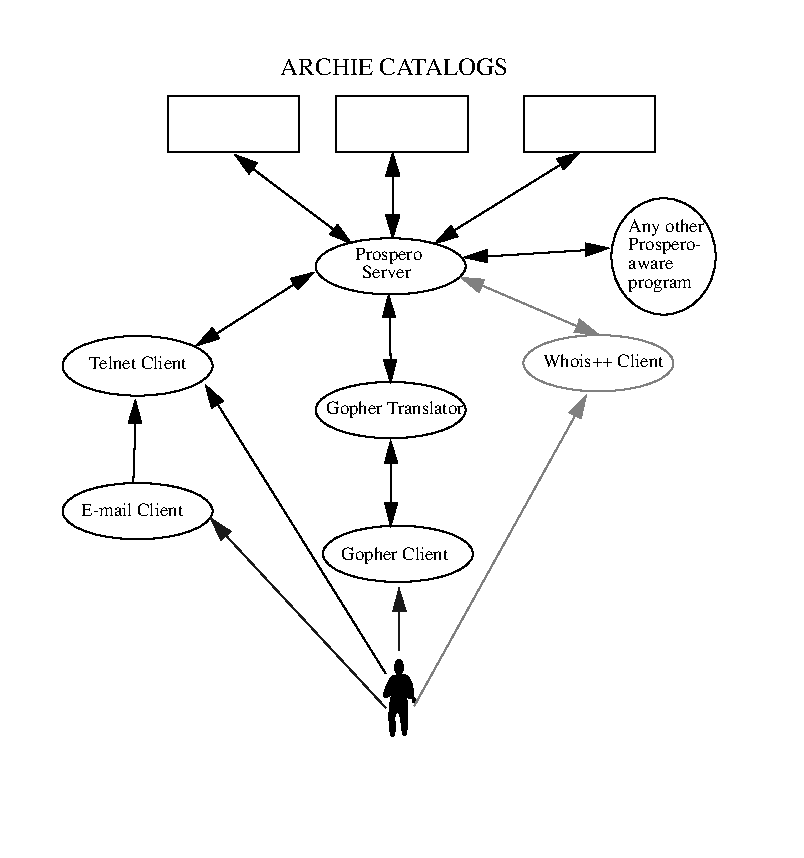
\epsfig{file=figs/catalogs.eps,height=4in}
\end{center}
\caption{User access to the Archie catalogs}
\label{fig:catalogs}
\end{figure}

The information provider aspect of the Archie system is shown in Figure~\ref{fig:catalogs}.
Originally, the Archie system used a modified Prospero File System server
({\bf dirsrv}) to provide user access to its catalogs.  Another module
has been added to the system to access the catalogs via WWW
browsers. \new


The Archie system catalogs are maintained by the Update Cycle processes shown
and described in the following pages. This is illustrated in Figure~\ref{fig:cycle}.


\begin{figure}[!htb]
\begin{center}
\epsfig{file=figs/cycle.eps}
\end{center}
\caption{The Archie update cyle}
\label{fig:cycle}
\end{figure}

Of more immediate importance to Archie system administrators is the
information-seeker aspect of the Archie system. This is composed of several
components which work together to retrieve, parse and update data in the
Archie databases, and is illustrated in Figure~\ref{fig:process}.


\section{Overview of the Archie Update Cycle}

First, some useful definitions:

\begin{itemize}

\item
The catalogs are the collection files which are consulted when a user
carries out an Archie search. For example, the anonftp catalog contains an
index of the files available from anonymous FTP archives on the Internet while
the webindex catalog indexes the WWW space.

\item
The term Data Hosts refers to those network sites which contain the
information that the Archie system will hold in its catalogs.

\item
The Host Information Files or Host Databases contain the latest information
about each of the Data Hosts and the data stored there. The Host Information
File Manager is responsible for maintaining these files.

\item
From the perspective of the Archie administrator, Archie servers fall into
two categories. The local Archie host (site, server) is the one that the
administrator is responsible for maintaining. Remote Archie hosts (sites,
servers) are all those other sites on which the Archie system is being run.

\item
Each component is controlled by a component manager.

\end{itemize}



The major steps of the Update Cycle are:


\begin{itemize}

\item
The Retrieval Component consults the Host Information Files to determine
which Data Hosts should be scheduled for inspection. This information is used
to start the Update Cycle; the rest of the Cycle is
concerned with accessing these sites and retrieving any new data.

\item
The Data Acquisition component is concerned with obtaining any new data
directly from the Data Hosts for which the Archie server is responsible.

\item
The Parse Component is responsible for parsing the incoming data into a form
suitable for the update of the Archie server's catalogs. This often means
removing extraneous information (filtering), as well as performing data
conversions, collation and compression.

\item
The Exchange Component obtains data from remote Archie
servers, if it has been configured to do so. Data so obtained is inserted into
an appropriate place in the Update Cycle and is ultimately incorporated into
the Archie catalogs on the local Archie host.

\item
 Finally, the Update Component obtains the parsed data and integrates it into
the appropriate Archie catalog files. This entails updating the catalogs with
the information obtained from the Data Hosts (or other Archie servers), as
well as making changes to the Host Information Files. Recall that the Host
Information Files contain information such as the last time a Data Host was
accessed for inspection; this information must be brought up to date at the
end of each Update Cycle.

\end{itemize}


Before describing the Update Cycle process in more detail, some important
concepts need to be described.

In order to carry out its processing, the Archie system must maintain special
information about the Data Hosts from which it gets information, and the
status of the information stored in the Archie catalogs that has been obtained
from those sites. These particulars are stored in files collectively referred
to as the Host Information Files. They are maintained by the host\_manage
program.

The Host Information Files fall into two categories: a primary information
file and (possibly) several auxiliary information files. These reside in


\path{\archie/db/host\_db/host-db.dir}

and

\path{\archie/db/host\_db/host-db.pag}


The primary host information file contains particulars about the physical Data
Host itself:


\begin{itemize}
\item the primary name of a site

\item the primary IP address

\item the operating system (if known)

\item timezone (if known)

\item access methods (catalog names)

\end{itemize}


\begin{figure}[!htb]
\begin{center}
\epsfig{file=figs/process.eps,height=6in}
\end{center}
\caption{The Archie system process interactions}
\label{fig:process}
\end{figure}


The Archie server also maintains auxiliary Host Information Files in


\path{\archie/db/host\_db/hostaux-db.dir}

and

\path{\archie/db/host\_db/hostaux-db.pag}


These contain details for a particular Archie catalog. For example, if the
Archie server is keeping track of the anonymous FTP listings of the site
bunyip.com, there would be an entry in the auxiliary files for
bunyip.com/anonftp.

These files contain, in part:

\begin{itemize}
\item The name of the Archie catalog (e.g., anonftp or webindex)

\item The preferred name (that is Domain Name System CNAME, if set)

\item Source Archie server

\item Time of last data retrieval

\item Time of last data parse

\item Time of last update

\item Number of records (catalog-specific definition)

\item Number of times an update has failed

\item  Any comment that the Archie system has seen fit to communicate to the
administrator (reasons for failure of update for example)

\item The current status of the information service at the Data Host (active,
inactive etc.)

\item The name of the Archie host responsible for monitoring this site (for
those cases in which the data is being exchanged between Archie hosts)
\end{itemize}

The Data Host Information Files are maintained by the host\_manage program,
which is described in ``Managing the Host Information Files'' on
page~\pageref{chap:hostmanage}.

Every piece of New Data introduced in the Archie Update Cycle begins with an
Archie header record. This contains all the information necessary for the
various components to process the data obtained from the Data Host. The
information in the header is modified throughout the Cycle to reflect the
changing status of the data. Much of the final information in the header
record is used to update the Host Information Files at the end of the
Cycle. While in most cases the Archie system administrator need not be
concerned with the header records of data within the Archie system, it is
useful to know what the record contains, if problems should occur.

In some cases, the header itself contains all the data necessary to complete
the Update Cycle. For example, for an Archie catalog describing the status
(reachable or unreachable) of sites on a network, an indication of ``success''
or ``failure'' in the header would be enough to know whether to proceed with the
update.

The header is in printable ASCII characters and is human-readable regardless
of the format of other data which may follow it. All headers start with
the string @header\_begin and are terminated with @header\_end. The data itself
starts immediately after the final NEWLINE of the termination string.

\alertbox{It is not advisable to edit Archie data files, especially if the
data is in binary form. Most text editors do not correctly handle binary
files.}

A description of the header can be found in Appendix~\ref{app:header}.
Currently, all header fields are optional, with the exception of the primary
hostname entry.

\section{Update Cycle file naming conventions}

All data files created and maintained during the Update Cycle have the
following naming convention:

\texttt{<primary site name>-<dbname>[\_<id number>].<phase suffix>[<temp>]}

\noindent where

\begin{TTentry}{<primary site name>}

\item[<primary site name>]
is the name of the Data Host.

\item[<dbname>]
is the name of the Archie catalog to be updated with this data.

\item[<id number>]
is an arbitrary number determined by components of the Update
cycle to prevent name clashes (i.e. when there is more that one set of data
associated with the \Param{<primary site name>/<dbname>} pair). Note that this is
OPTIONAL and may not occur in certain file names.

\item[<phase suffix>]
is one of retr, parse or update specifying which part of the
update cycle the data is destined for, not from which the data came.

\item[<temp>]
is a string appended to the name if the current file has a temporary
status, i.e. is undergoing a data transformation (such as being
uncompressed). Currently this is ``\_t''.

\end{TTentry}

\noindent An example using this naming scheme is:

\path{bunyip.com-anonftp\_54.parse\_t}


\alertbox{All files undergoing processing are stored in the \archie/db/tmp
(``holding'') directory, unless otherwise specified (using the ``-t'' switch).}


\alertbox{The manual pages describe how to override the default holding
directory for the Archie programs. However, the directory you choose instead
of \Path{\archie/db/tmp} must not be on a different filesystem (partition) from
\archie, as the programs make use of ``hard links'' which cannot cross partition
boundaries. See ln(1).}



%
%
%
\section{Process naming conventions}

By reading the header record the controlling process of Archie's Update Cycle
automatically generates the name of the appropriate program to invoke for the
successive phases in data processing. The syntax for the process name is

\path{<component name>\_<dbname>[\_<os type>]}

\noindent where

\begin{TTentry}{<component name>}
\item[<component name>] is one of retrieve, parse, update or net

\item[<dbame>]
is the name of the Archie catalog with which this data is associated

\item[<os type>]
is optional and is used when different operating systems require
different processing functions (e.g., when parsing a UNIX, Novell or
VMS anonymous FTP listing).
\end{TTentry}


For example, if the control program reads a header which specifies that this
data is destined for an anonymous FTP catalog, and that it requires parsing,
the control program will invoke the parse\_anonftp program. This program may,
in turn, look at the header and determine that it is a UNIX BSD listing and
will invoke parse\_anonftp\_unix\_bsd on the data file for processing.


\alertbox{There will be cases in which the operation to be performed is
similar enough that the same program may be used for more than one purpose. In
this case soft links, which follow the naming convention, are made
to a single program.}

The update process is complex and requires consistent and complete information
in order to complete successfully. This means it is possible to have a failure
at any step in the Update Cycle. For example, the data host may not be
reachable, or the parsing of the obtained data may fail. In this case, the
program will produce a file containing a header reflecting the nature of the
failure. This usually contains an explanation of how or why the failure
occurred (this is signified in the header record by the comment field). The
``failed'' data continues to be passed through the Update Cycle and at each
phase the header is updated to reflect what has happened to it. Thus, even
though the data acquisition has failed, the last\_parsed field of the header
will be updated.


%
%
%

\section{The Update Cycle in detail}
\label{sec:update}
Now, each component of the Update Cycle will be discussed in some detail.

The Update Cycle is performed, step by step, under the guidance of the
arcontrol program. It is invoked in different modes depending on the phase of
the Cycle desired. It scans the holding directory for the appropriate data
files and may perform some basic data transformations on those files (such as
uncompressing the data) before passing them on to the appropriate programs for
processing.

The steps followed by the system are as follows:


\subsection{The Retrieval Component (arretrieve)}

This component is responsible for querying the local Archie system for the
list of sites scheduled for inspection. It does so by contacting the local
Archie arserver process (see ``The arserver program'' on page 34) and
downloading a set of headers corresponding to those Data Host/catalog
combinations. Each header is placed in a separate file, ready for the Data
Acquisition phase of the cycle.

\subsection{The Data Acquisition Component (arcontrol -r)}

arcontrol examines the header files (created by the Retrieval Component). For
each Data Host/catalog pair, it determines the appropriate process for
retrieving new data for the catalog from the Data Host. arcontrol invokes the
selected process, passing the name of the header file as a parameter. Once the
process has finished acquiring information from the Data Host, a file
containing the results will be created (according to the scheme outlined in
``Update Cycle file naming conventions'' on page 23). The file will contain the
header record and either retrieved data or an indication of failure.

\subsection{The Parse Component (arcontrol -p)}

Managed by arcontrol, the processes responsible will parse the files generated
by the Data Acquisition Component into the appropriate form for the target
catalog. For example, in the case of anonymous FTP listings, it will take the
raw data and create an output file of the correct form for insertion into the
anonftp catalog.

\subsection{The Update Component (arcontrol -u)}

Invoked by arcontrol, the Update Component process performs two functions: it
will update the Host Information Files, and it will update the Archie catalog
itself. For example, when a correctly parsed anonftp (anonymous FTP) listing
from bunyip.com is ready, the data itself is inserted into the anonftp catalog
and the record for ``bunyip.com.anonftp'' is modified in the auxiliary Host
Information Files.


\section{Data Exchange}

This release of Archie allows the exchange of arbitrary catalog data between
cooperating Archie systems. A basic flooding i-have/send-me algorithm, similar
to that used in the Internet USENET news system, is used to maintain weak
consistency between an arbitrary number of Archie servers. ``Virtual'' networks
of Archie systems can be created and any individual server may belong to zero
or more of these data-exchange networks.

This allows a multi-tiered system (such as the example on the map) whereby
certain key sites may be responsible for inter-continental data exchanges and
others would feed from them, instead of every Archie site having to contact
all others worldwide.




\section{Conclusion}

This concludes the description of the Archie Update Cycle processes. With a
better understanding of how Archie works, you should be now be ready to
configure your Archie server to fulfill your needs. The discussion of Archie
configuration begins in section~\ref{chap:configure}, ``Configuring the Basic System'' .



%
% Copyright (c) 1996 Bunyip Information Systems Inc.
% All rights reserved
%
% Archie 3.5
% August 1996
%
% db.tex
%




\chapter{The database}
\label{chap:db}
\new

\section{Overview}

The database has been completely revised. The goals of this reconstruction
were the building of a faster system and more reliable database.  The back-end
of the database is composed of


\begin{itemize}
\item Index
\item Site files
\item Start database
\end{itemize}


The index is a tree structure, allowing fast searches of the strings file.
Rebuilding the index is a relatively expensive process, so it is not updated
after every new key is inserted into the database.  Thus, in order to handle a
search request, a linear search is made of the (usually) small un-indexed
portion of the strings file, in addition to checking the fast index.  To
ensure quick response times, the index should, periodically, be brought up to
date with the strings file.


Within a catalog, files having the prefix \Path{``Stridx.''}, are part of
the index.  For example, \Path{Stridx.Strings} is the strings file, and
\Path{Stridx.Index} is the fast index. Depending on the database, the
creation of the index is done differently. The anonftp database creates an
index file for all substrings where instead the webindex database creates
an index file that contains only the left substrings. 


The site files are now independent of one another. In case of corruption, only
the site that is corrupted need be considered. In certain cases, such as
webindex, extra files may be present with each site file. The
\Path{.excerpt} files contain excerpts of the different URLs.
The \Path{.idx} files, present in both anonftp and webindex, hold extra information
for large site files, in order to speed up searches.

The directory \Path{start\_db}, present in each catalog, holds information
that ties the index with the site files.

\section{Building the index}


In order to rebuild the index, the program \Path{db\_build} must be run.

The build may take some time to run, depending on the size of
\Path{Stridx.Strings} and the amount of memory allocated to the build.
One would call \Path{db\_build} as follows:

\comm{db\_build -d anonftp -v -k 50000 -t \archie/db/tmp }

The above example builds the anonftp index using 50 megabytes of memory.
Temporary storage is used in the \Path{\archie/db/tmp} directory. The man page lists
all the other switches that can be used. One option of particular importance
is ``\Comm{-f}'', which forces the index to be rebuilt, even if the un-indexed
portion of the strings file is very small. By default, the program will not
rebuild the index if the un-indexed text is less than 1 megabyte.

\alertbox{The index file is not constructed the same for each database. In the
case of the anonftp database, the index includes information concerning every
substring present in the string file. In the case of the webindex database,
the index is built for every word prefix present in the string file, i.e.
all substring that start at the beginning of a word.}


\alertbox{You may want to rebuild the index once a week initially and then
only once a month. These estimates are speculative --- it depends
on the rate at which new strings are added to the database.}

\section{Ordering the results}

With the volume of information in the database and the amount of replication
on the network, it is often desirable to return the results in some order of
closeness. It is now possible to configure the order in which results are
returned, according to the name of the domain to which the result site
belongs. To avoid slowing down searches, this ordering is done at the time at
which the data site is inserted into the database, rather than when the
results are being returned.

The order is defined in the file \Path{\archie/etc/domain.order}. The
following is an example of such a file.

\begin{center}
\begin{tabular}{l}
\Param{\# Comment line} \\
\Param{\# Domain order for an Archie server in North America} \\
\Param{ca:edu} \\
\Param{com:gov} \\
\Param{*} \\
\Param{au:nz} \\
\end{tabular}
\end{center}


Domains on the same line have the same precedence. Hence, \Param{.edu} sites
and \Param{.ca} sites will be returned first, in no particular relative order.
The sites in the domains \Param{.com} and \Param{.gov} will be listed later.
To discourage users from making unnecessary, long distance file transfers, the
sites from New Zealand and Australia are returned last. (We assume that users
accessing a North American archie server are usually in North America.) The
``*'' represents all other sites.

One can also specify the domains using pseudo-domains defined in
\Path{\Archie/etc/ardomains.cf} as well as sub-domains such as \Param{bunyip.com}.

\alertbox{For a given keyword in the database, the list of sites in which it
belongs is ordered. The result of this is that the answer returned from a
search may seem unordered.
In fact, the list of results is composed of sub-lists, each one for a
specific keyword matching the search criteria, and each one of 
those sub-lists are ordered according to the specified order.
Note also that some clients such as xarchie reorders the results and you may
not get the results in the appropriate order.
}

\alertbox{In order for changes, in the order of domains, to take effect, you must
rebuild the precomputed orders for the existing sites. This is done with the
program \Comm{db\_reorder}, listed in section~\ref{sec:programs}. }

\alertbox{Note that there are no leading dots ``.'' in the listed domains}




\section{The other programs}
\label{sec:programs}

All programs prefixed by \Path{db\_} in \Path{\archie/bin} aid in managing the
database. They are:

\begin{center}
\begin{tabular}{|l|l|} \hline
Program & Description \\ \hline\hline

db\_build & Build the database index \\ \hline
db\_check & Verify the consistency of the database \\ \hline
db\_dump  & Dump the list of sites that are in \Path{start\_db} \\ \hline
db\_reorder & Reorder the sites according to \Path{domain.order} \\ \hline
db\_siteidx & Build the \Path{.idx} files for specific sites \\ \hline
db\_stats & Compute statistics \\ \hline
fix\_start\_db & Fix problems in the start\_db database. \\ \hline
\end{tabular}
\end{center}

Information about the command line options of these programs may be found in
their respective man pages.






%
% Copyright (c) 1996 Bunyip Information Systems Inc.
% All rights reserved
%
% Archie 3.5
% August 1996
%
% install.tex
%

\chapter{Installing the basic Archie system}
\label{chap:install}

This section will guide you through the process of installing the Archie
software on your system. With an understanding of the overall Archie system
architecture, as presented in chapter~\ref{chap:overview}, we will then proceed
to the configuration of the system.


\section{Archie system space requirements}


Choosing a location for the Archie system on your file system depends
on the databases that you intend to maintain. We estimate that a complete
{\bf anonftp} catalog (covering about 1200 archive sites) requires
between 600 and 1000 megabytes. In the case of a {\bf webindex} catalog,
the space requirements are as much as possible!  

To help decide on the location of the Archie system, let's take a look
at the directory structure that will be created once the distribution
is unpacked.

\begin{center}
\begin{tabbing}
Directory/file pathname\hspace*{5mm}\= Purpose \\
\\
archie/ \> Archie system home directory \\
archie/cgi \> CGI related directories \\
archie/cgi/bin \> CGI binaries \\
archie/cgi/html \> HTML files \\
archie/contrib/ \> public domain and third-party software \\
archie/config/ \> installation configuration \\
archie/bin/ \> system binaries and shell scripts \\
archie/db/ \> Archie database home directory \\
archie/db/anonftp\_db/ \> anonymous FTP catalog files \\
archie/db/webindex\_db/ \> WWW catalog files \\
archie/db/host\_db/ \> host database files \\
archie/db/locks/ \> directory for lock files \\
archie/db/tmp/ \> temporary or ``holding'' directory for data files \\
archie/doc/ \> system documentation \\
archie/etc/ \> system configuration files \\
archie/help/ \> Archie client help directories and files \\
archie/logs/ \> system log files \\
archie/logs/archie.log \> main Archie system log file \\
archie/logs/email.log \> log file for email client (if installed) \\
archie/manpages/ \> Archie system manual pages \\
archie/pfs/ \> Archie/Prospero system home \\
archie/pfs/bin/ \> Archie/Prospero binaries \\
archie/pfs/pfs.log \> Prospero log file  \\
\end{tabbing}
\end{center}

The directories \Path{db/tmp}, \Path{db/anonftp\_db} and
\Path{db/webindex\_db} will likely use the most space. Previous versions of
the Archie system required that those directories be part of the same disk
partition. The current version removes that restriction. \new The only
limitation still present, in this version, is the requirement that
\Path{db/tmp}  and 
\Path{etc} still be in the same partition. The catalog directories may reside in
separate partitions.



%
% Archie user codes 
%

\section{Archie user codes}


Two user codes need to be created to enable Archie system operation and
maintenance. The first, called {\it archie}, is used for non-administrative
access to the Archie system (e.g., for accepting user queries to the Archie
databases). The second, called {\it archuser}, is for system maintenance by
the Archie system administrator. The password file entries for these two users
should specify, in the home directory field, the full path to the root of the
Archie system. The password file entries for these two codes also should meet
the following requirements:


\begin{itemize}

\item
both codes must have the same UID (User ID) number

\item
NEITHER code should have any special privileges, such as belonging to the
wheel or staff groups

\item
the archie user code must appear {\it before} the archuser code in the password
file

\item
the archuser code should have whatever shell you normally use (e.g.
/bin/csh or /bin/ksh)

\item
the archie user's shell field should be set to /bin/false for the time
being. This will be changed if a telnet client is installed
(See ``Setting up the anonftp catalog clients'' on page~\ref{chap:clients}.)

\item
the password field for archie should be set to asterisk (`*') for now. This
will be changed if you install the Archie telnet client
(See ``Setting up the anonftp catalog clients'' on page~\ref{chap:clients}.)

\item
The password field for the archuser code should be set to one of your choosing

\item
The \Path{/etc/group} file must be modified to create a group named ``archie''
for the Archie user codes. For example:

\texttt{archie:*:1000:archie,archuser}

\item both codes must have the same GID (Group ID) number in the password
file, and this must be the number, set above, for the archie group.

\end{itemize}

Thus, an example of the entries in the \Path{/etc/passwd} file is:

\texttt{archie:*:23:1000:archie client code:/usr/local/archie:/bin/false}

\texttt{archuser:ufUn9Ap.:23:1000:archie admin code:/usr/local/archie:/usr/bin/csh}


If you are using the Network Information System (NIS) you should only need to
add the above entries to the /etc/passwd file for the local Archie host, not
for the entire NIS system.

\alertbox{The naming convention of \archie \ or \Path{\Archie}
is used here to specify the home directory of the Archie system.}





%
%
%

\section{Unbundling the distribution}

This new version of Archie contains not only a new set of binaries and a new
catalog, but certain elements, internal to the system, also have been modified.
If you already have an existing Archie installation, the catalogs will
have to be rebuilt. \new Fortunately, you can convert the existing host\_db database
to the new format.

\alertbox{If you are upgrading your software from version 3.3 and want to
save the host database, you will need to make a backup copy of the directory
\Path{\archie/db/host\_db}. Be sure to read section~\ref{ndbm} before
proceeding with this.


Once you have installed all the software, restore the host database
then run the program \Path{convert\_hostdb}, as follows:

\comm{convert\_hostdb}

The new host database will then be converted and will contain only
those sites for which you are responsible (i.e. that you retrieve).
}
\new 


First start by FTPing the distribution from ftp.bunyip.com. In the directory
archie-\version \ you will find the files that need to be retrieved.

\begin{itemize}
\item archie-\version-install.tar 
\item archie-\version-arch-version.tgz 
\item archie-\version-arch-version-A.tgz 
\item archie-\version-arch-version-B.tgz
\end{itemize}

where ``arch-version'' is one of: `sunos-4.1.4', `sunos-5.4', or `aix-3.2'.

Untar `archie-\version-install.tar' with the command:

\comm{tar xvpf archie-\version-install.tar}

There you will find three scripts that will be used to install the binaries,
`unwrap', `untar', and `unrotate'.  The single command, `unwrap' should take
care of installing the binaries and other files.


To install the server software, as superuser, type:

\comm{./unwrap}

and follow the instructions. As indicated by the script, you need to
set the correct permissions. If you want to install the Archie man pages
in a system-wide area, read the next section. As superuser type:

\comm{cd \archie/config}

\comm{make}



This will change the permissions of the files in the Archie system to the
appropriate values, as well as install the manual pages into the directory
specified above.

In addition, a symbolic link will be created from the root directory pointing
to the Prospero tree. Typing

\comm{ls -al /pfs}

will show you the link and the directory to which it points. It will look
similar to:

\param{lrwxrwxrwx 1 root 33 Mar 2 23:28 /pfs -$>$ /usr/local/archie/pfs}



It is suggested that the installation and configuration be performed as the
user archuser except for those changes that must be made as the superuser.



%
% Man pages 
%

\section{Manual Pages}

The on-line manual pages are, by default, configured to be installed in the
Archie man directories \Path{\archie/man}.
However, you may opt to install the man pages in a different location,
as described below.

First
\Path{cd \archie/config} and edit the file
\Path{Makefile}. Modify the line:

\path{MAN=../man}

to be the name of the directory where you would like the Archie system
manual pages placed, if it is different from the existing location.

Change the line:

\path{MANEXT=n}

to reflect the manual page name extension for that directory.

For example, if you wanted to store the Archie manual pages with the system
man pages, you could change the appropriate lines, as follows:

\path{MAN=/usr/man/mann}

\path{MANEXT=n}



If the manual pages are placed anywhere other than your system's default manual
directories, you may have to change your UNIX environment variable MANPATH to
reflect the changes. Otherwise, the \Path{man} command will not find the Archie
manual pages.



\section{ndbm and Berkeley DB files}
\label{ndbm}
\new

In the previous versions of Archie, ndbm files were used to maintain certain
information on hosts etc. It, now, uses Berkeley DB library to construct and
maintain those databases.  These files have extension \Path{.db}.

%
% Congratulations
%

\section{Done !}

You have now finished the initial installation of the Archie system. The next
section  will describe how to configure the system. You may want, first,
to reread the overview section~\ref{chap:overview} to understand the different
aspects of Archie.






                     % Installing the basic Archie system.
%
% Copyright (c) 1996 Bunyip Information Systems Inc.
% All rights reserved
%
% Archie 3.5
% August 1996
%
%  Configuring the Basic System
%



\Chapter{Configuring the Basic System}
\label{chap:configure}

Now that you have an understanding of the basic structure of the Archie
system, you are ready to continue with the configuration procedure. The
sections in this chapter deal with the necessary installation fine tuning that
will allow you to configure your Archie system to behave appropriately in your
environment.

\section{Configuring the pseudo-domains database}

A pseudo-domain is an alias for a set of domain names. Pseudo-domains are
useful for describing a collection of Domain Name System (DNS) domains which
may not apparently be related (e.g., by spelling). For example, ``.usa'' may be
defined as ``.mil'', ``.com'', ``.edu'' and ``.us''.

The Archie system makes use of pseudo-domain definitions. This is primarily
for convenience in specifying domains as catalog search constraints. The files
\Path{\archie/db/host\_db/domain-db.\symbol{123}dir,pag\symbol{125}}
contain the information where these
definitions are stored. It is the responsibility of individual Archie system
administrators to configure these files as necessary. Note that this database
is visible from remote Archie clients (for example in the anonftp
telnet-client the domains command allows users to see the domain structure of
a server). Users may also search within the catalogs using these pseudo-domain
definitions as restriction criteria.

The tool for modifying this database is the ardomains program, found in
\archie/bin. The input to this program is a file following the format in the
example (see below). The example and the default configuration file are
provided as illustrations of the appropriate format. Some modification will be
necessary to tailor the setup to your Archie server environment.

\begin{center}
\begin{tabular}{lll}
\multicolumn{3}{l}{\#This is a comment line} \\

europe      &  de:ie:pt:es:uk:at:fr:.il:be:nl:ch  & Europe \\

scandinavia  &  no:dk:se    &                       Scandinavia \\

northamerica &  edu:com:gov:us:ca:mil &              North America \\

asia   &      kr:hk:sg:jp:cn:my:tw:in  &          Asia \\

world &       europe:scan:noram:asia    &         The world \\

\end{tabular}
\end{center}

In the example, the pseudo-domain europe has been defined to include the root (top-level) DNS domain names (ISO codes) of the countries of Europe. Pseudo-domain definitions can be nested. So, for example, world is composed of the pseudo-domains europe, scandinavia, northamerica and asia. Short descriptions (265 characters or less) of the pseudo-domains may optionally follow their definition.

When determining if a specific site is a member of a particular pseudo-domain, the Archie system iteratively resolves each pseudo-domain into its base constituents. Thus, world is broken down as follows: 

\path{europe:scan:noram:asia}

and in turn, europe is taken as:

\path{de:ie:pt:es:uk:at:fr:.il:be:nl:ch}

The Archie system then searches to see if any of these are, in turn,
pseudo-domains. This process can be nested to 20 levels.

If an entry cannot be resolved into subcomponents, it is taken ``as is''. Thus
for example, the pseudo-domain uquebec could be arbitrarily defined as

\path{uquebec mcgill.ca:uqam.ca:concordia.ca:umontreal.ca Universities in Quebec}

This provides a list of the various domains within the pseudo-domain of universities in Quebec. The mcgill.ca string cannot be further resolved by the system, so it is considered a base component.

This technique gives both the Archie administrators and users a shorthand notation for specifying domains.

The following points should be kept in mind:

\begin{itemize}
\item
Pseudo-domains must be defined before being used in other pseudo-domains.

\item
On final resolution, the names must match a real DNS domain. The Archie system
makes no attempt to verify the authenticity of the base domains: they are just
used for comparison with site names. A non-DNS name will never successfully
match any data host names stored in an Archie catalog.

\item
The Archie system carries out comparisons of domain strings from right to
left. Thus, m.ca matches both crim.ca and uqam.ca. This can be used to
advantage in constructing domain specification strings. In the example above,
the .il entry differs from the rest by having a preceding period (``.''). This
is so that sites in Israel (``.il'') do not match US military sites (``.mil'').
\end{itemize}


\subsection{Loops in the domain database}

The system will detect domain ``loops''. For example, the entries


\path{canada  qc.ca:on.ca  Provinces in Canada}

\path{on.ca   canada       Ontario}


form a loop: canada resolves into on.ca and qc.ca; on.ca refers back to canada. Archie administrators should try to avoid introducing such loops in their specifications. The ardomains program will identify any it detects.

\subsection{Building the domain database}

To create the domain database, run the program \archie/bin/ardomains on a file containing entries as specified above. The syntax is:

\comm{ardomains [<input file>]}

The \Param{<input file>} should reside in \Path{\archie/etc} for future
reference by Archie programs. By default, the file \archie/etc/ardomains.cf is
used if no file is explicitly given. A sample file is provided in the
distribution for your convenience. Please consult the manual pages for full
details on using this program.



A backup copy of the domains database is maintained in the
\Path{\archie/db/host\_db} directory. Thus, the system is never without a
domain database, even when ardomains is completing the update procedure on the
domain database.



\subsection{Files used by ardomains}

\begin{center}
\begin{tabular}{lll}
File Name & Type & Description \\

\archie/bin/ardomains & Executable & ardomains program \\

\archie/db/host\_db/domain-db.\{dir,pag\} & ndbm data & main domains database
file \\

\archie/db/host\_db/domain-db-new.\{dir,pag\} & ndbm data &
active domains database file (hard link to above) \\

\archie/db/host\_db/domain-db-old.\{dir,pag\} & ndbm data & 
previous version of domains database \\

\end{tabular}
\end{center}


\section{The arserver program}
\label{sec:arserver}

The arserver program provides the external Internet world with a view of the local Archie Host Information Files. It is responsible for responding to queries about the Data Host information as well as performing the protocol negotiations necessary for inter-Archie data exchanges. The server is designed to be run by the UNIX inetd process and thus the file /etc/inetd.conf needs to be modified to inform inetd about the new process.

\alertbox{You must be logged in as superuser to carry out these changes. }



The following single line must be added to the /etc/inetd.conf file with the
correct entry for \Archie \  (the Archie home directory):

\param{arserver stream   tcp  nowait  archuser	 \Archie/bin/arserver  arserver  -l}

The following line should be added to the /etc/services file:

\param{arserver  2710/tcp}

\alertbox{2710 is not a reserved port number. Future releases will probably make use of a reserved port.}



\alertbox{If your system is running the Network Information Service (NIS, formerly called Yellow Pages), additional steps must be taken to incorporate the new services file in your system. Please refer to NIS documentation for details.}



Once these changes have been made, inetd must be notified. The easiest way to
do this is to restart the inetd process. In SunOS 4.X, this can be
accomplished as follows:

\comm{ps aux | grep inetd}

This will extract a line specifying the inetd process, which will look like:


\param{root 162  0.0  0.0  52  0  ?  IW  Oct 23 0:30 inetd}



The process number (\Param{<procnum>}) is the second field (in this case 162). 



Then issue the command:

\comm{kill -HUP <procnum>}

This tells the inetd process to re-read the (modified) configuration file.

For an RS6000 system, however, the following command will perform the necessary updates:

\comm{inetimp; refresh -s inetd}


\section{Invoking arserver}

There are three programs associated with transferring data site information
between remote Archie servers, and internally within your own local Archie
server. They are:

\begin{itemize}
\item arserver

\item arexchange (inter-Archie exchange)

\item arretrieve (local Archie updates)
\end{itemize}


\alertbox{arexchange and arretrieve are currently soft links to the arserver
program; the different names serve to distinguish between tasks to be
accomplished.}



The arserver program is designed to run on demand as connections are made to
it. The arexchange and arretrieve programs, however, are to be run
periodically. This process can be automated through the use of cron (see the
UNIX manual entry cron(8) for details).






\alertbox{All entries for cron should be made in the archuser crontab file, since archuser is the administrative code for the Archie system. Failure to do so may cause problems with improper file permissions for the data files and executable programs.}





All examples in this section will refer back to this sample file. The
arcontrol program will be described in greater detail in ``Controlling the
Update Cycle'' on page~\pageref{sec:control}.



\begin{figure}[!htb]
\begin{center}
\epsfig{file=figs/exchange.eps,height=2.8in}
\end{center}
\caption{arserver, arretrieve and arexchange relationships}
\end{figure}




%
%
%

\section{Configuration}
\label{sec:configuration}

The arserver, arexchange, and arretrieve commands make use of two
configuration files, with which the Archie system administrator can configure
such things as the data sites that are to be inspected for updating Archie
catalogs (in arretrieve.cf), or the remote Archie servers that are permitted
to participate in an exchange of information (in arupdate.cf).

arupdate.cf is consulted by both arserver and arexchange, while arretrieve.cf
is consulted by arretrieve. Both reside in \archie/etc. Both files have the
same format, but different semantics.






\alertbox{Please note that both configuration files are overwritten by the process accessing them (arretrieve.cf by arretrieve and arupdate.cf by arexchange) at the end of processing. Changes written to the configuration files by the administrator while the processes are running will be lost. }



The Archie site administrator is responsible for configuring these two files
so that the system performs the desired local data retrievals, in addition to
remote exchanges with other Archie hosts.


\section{Configuration decisions}

There are a number of factors to be considered when performing the configuration:

\begin{itemize}

\item What data do you want to store in your local Archie system? This
means deciding which catalogs you would like to serve and from which Data
Hosts you want to pick up the information. For example, you may decide that
you would like to serve all anonymous FTP sites (the anonftp catalog) in
Nigeria, Mongolia and Barbados or provide a webindex catalog for all of
Europe.

\item With whom do you want to exchange inter-Archie data? If you are in a remote location from the data that you would like to serve to your user community, you will probably find that somebody closer is already collecting this data. It is possible that they will be interested in exchanging data with you as well.

\item How often does the data, that you are going to collect yourself or
exchange with a remote Archie site, change? There is no need to exchange
information frequently when the data itself changes infrequently. This also
wastes network bandwidth that could be better utilized.

\item With the current version of the Archie system, the minimum amount of
time between inspections of a Data Host must be greater than the amount of
time required to complete the Update Cycle from the last access. This is
because the Host Information Files are updated as the last step of the Update
Cycle, so the information that would be used to start the next Update Cycle is
not yet available.
\end{itemize}

%
%
%
\section{Choosing Data Hosts}

The worldwide Archie system generally works as a set of independent,
cooperating providers, serving the Internet community. While most Archie
servers are primarily interested in serving their local community on the user
query side of the system, the data host information exchanged between servers
allows each system to provide global data, while only having to monitor a
relatively small number of local data hosts. Each server is free to collect
data directly from any data host desired, however cooperation in the general
data exchange network benefits all concerned and is encouraged.

You may choose to gather data from Data Hosts directly, while obtaining the information about other data hosts from other Archie systems. You should decide which data hosts, if any, you are interested in contacting directly for information and which you would like to obtain from remote Archie servers. Once this decision is made, you can configure your system appropriately.



\alertbox{Bunyip Information Systems coordinates Archie exchanges among its customers as part of the annual support agreement.}



The Archie administrator has significant control over the criteria used to determine what is updated and how often. For example, the Archie system can be configured so that nearby sites are inspected every day while more remote sites are checked every two days. Alternatively, it can be configured so that certain catalogs are updated on even days, and others on odd days. Inter-Archie data exchanges can be configured in a similar fashion.

The next sections will describe the precise format and semantics of the configuration files.


%
%
%
\section{The Retrieval Phase}

As mentioned earlier, the Retrieval Phase is the first step in the Update
Cycle. The local Archie Host Information Files are queried through the use of
the arretrieve command. The query is composed of a set of criteria (or
constraints) that the specified Data Hosts need to meet in order to be
inspected. (For a detailed description of the protocol used between arretrieve
and arserver, see the manual page archie\_protocol). arretrieve then requests
that header records be obtained for any Data Hosts that meet the specified
constraints. These are deposited in the holding directory, where they await
the next phase of the process (refer back to ``Header Records'' in
Appendix~\ref{app:header} for more information about Archie system headers).



The queries that arretrieve sends to arserver are based on the information that the Archie administrator has set up in the arretrieve.cf file. 

\param{<the\_entry>:= <arserver host> <config line>}

\param{<config line>:= <config line> <config> | <config>}

\param{<config>:= <db list> <domain list> <max no> <perms> <freq> <date> <fail>}

where

\begin{TTentry}{<arserver host>}

\item[<arserver host>]
is the Fully Qualified Domain Name (DNS) of the host running the arserver program, to which the arretrieve client will connect. arretrieve and arserver may be run on different machines. However the majority of the time this entry will be localhost.

\item[<db list>]
is the colon (``:'') separated list of Archie catalogs which are to be retrieved.

\item[<domain list>]
is the colon (``:'') separated list of domains and pseudo-domains which the Data Hosts need to match in order to be returned. 

\item[<max no>]
is the maximum number of sites returned matching the criteria.

\item[<perms>]
Permissions (`r'ead or `w'rite). Must be `w' to enable transfer. A value of `r' effectively converts this line into a comment: it will be read but no action will be taken.

\item[<freq>]
A number specifying the minimum number of minutes that are to elapse before contacting arserver with this query again. It may have the modifiers `h' or `d' immediately following the number, specifying that the value is in units of hours or days respectively.

\item[<date>]
Date in YYYYMMDDHHMMSS format. Typically, this specifies the last time that the program performed such a query. In fact, the date is determined by the date of the most-recently inspected site. This is explained more fully in ``Dates in the configuration files'' on page 43.

\item[<fail>]
0. Ignored by arretrieve.
\end{TTentry}

The character \symbol{92} in the configuration file indicates that the entry is continued on the next line of the file.

The following example illustrates the format:

\param{localhost anonftp mcgill.ca:uqam.ca 30 rw 12h 19920703162322 0\symbol{92}}

\param{\hspace{10mm}whois:yp bunyip.com:cndir.org 30 rw 30d 19920603162322 0}

This can be explained as follows:
\begin{center}
\begin{tabular}{|l|p{3in}|} \hline
Field Content & Description \\ \hline \hline

localhost & Contact the arserver program running on the same host as the
arretrieve program. This is the case in almost all Archie installations. \\ \hline
 
anonftp & specifies that information for the anonftp catalog is to be
inspected. Alternatively a `*' may be given, signifying all catalogs. \\ \hline

mcgill.ca:uqam.ca & specifies that they are only to be from sites in the
mcgill.ca and uqam.ca domains. Any pseudo-domain definition may also be
given. Alternatively, a `*' may be given signifying all domains. \\ \hline

30 & specifies that at most 30 sites are to be returned on the retrieval. \\ \hline

rw & The `w' specifies that this line is ``enabled''. The `r' is ignored. \\ \hline

12h & specifies that the program should contact arserver every 12 hours \\ \hline

19920703162322 & specifies the last time arretrieve queried arserver about
this \Param{<database list>/<domain list>} combination. For the initial configuration,
this should be set to your current date and time. The client queries the
server for ``all sites that have not been inspected since \Param{<date>}''. \\ \hline

0 & 
is ignored by the client and should be set to 0 \\ \hline
\end{tabular}
\end{center}

The \symbol{92} signifies that the entry is continued on the next line.

The second (continuation) line gives a configuration for catalogs called whois and yp.

In this way, the Archie system administrator can completely configure how often sites are to be inspected, with full control over what is returned. For example, if one wanted to be responsible for (and query) all Canadian and American sites every day for anonymous FTP information, but European sites only once a week, the configuration could be:


\param{localhost anonftp ca:usa 40 rw 1d 19920810162322 0 \symbol{92} }

\param{\hspace{10mm}anonftp europe 30 rw 7d 19920810162322 0}

This example is only an illustration. In most cases, one would not be responsible for such a large region directly, but would pick up such information through data exchanges with other Archie servers.

The example illustrates a case where the Archie administrator wants to inspect data hosts less frequently than those on the same continent as the Archie server. Specifically, anonymous FTP archive sites within Canada and the United States are to be inspected every day, while those in Europe are to be inspected only every 7 days. 

arretrieve is designed to be run from the cron(8) daemon with a frequency no less than that specified by the shortest interval in the configuration file frequency field.

In the above example, the shortest interval specified is 1 day. The following line would be appropriate in the crontab(5) file.

\param{15 2 * * * \Archie/bin/arretrieve -l -M \Archie/db}

This specifies that cron is to run the arretrieve program at 2:15 every
morning. All appropriate inspections will be started up at this point. In the
example given, North American sites will be inspected each day, and the
European sites will be inspected only once every 7 days. \Archie, is of
course, the Archie home directory. See crontab(5) for full details on the
format of the file.


The arretrieve program does not retrieve any headers.

\NOTE

\begin{itemize}

\item For initial configurations ensure that the date field in the arretrieve.cf file is set to the current date.

\item The first field of the arretrieve.cf file, in almost all cases, will be the special name localhost. Check to make sure that this is the case in your configuration file.

\item Re-check the configuration file to be sure that the syntax is correct and that domains and catalog names can be resolved.

\item Check that arretrieve is a soft link to the arserver binary and that the archuser code has read/execute permissions on the file. 

\item Check that the arretrieve.cf file is has read/write permission for the archuser code.
\end{itemize}



%
%
%

\section{Inter Archie data exchange}

The local arserver program will accept connections from remote arexchange
clients. Similarly, the local arexchange program can contact those remote Archie
arserver programs that give it permission. These permissions are
defined in the configuration file. The default configuration file is
\archie/etc/arupdate.cf. As noted earlier, this configuration file has the
same format as arretrieve.cf, but the semantics are different.

Through the arupdate.cf configuration file, you can set up both symmetric and asymmetric exchange procedures. The symmetric relationship occurs when the connections to your Archie peers are bi-directional: you retrieve data from them and they from you. The asymmetric relationship occurs when either you only retrieve data from them (and not they from you) or vice versa. This is controlled through the use of the \Param{<perms>} field, described below.



\alertbox{Arrangements for the client/server connection must be enabled by the administrators on both sides of the connection for it to be successful. Bunyip regularly posts contact information for Archie servers worldwide on its support mailing lists.}



\subsection{The arupdate.cf file as seen by arserver}

For arserver, the configuration file provides a simple but effective security
mechanism which allows only those sites who have previously been given
permission, by the local administrator, to contact that server.

The fields in the configuration file have the following meanings to arserver:

\begin{TTentry}{<domain list>}
\item[<client host>]
is the Fully Qualified Domain Name (FQDN) of the remote Archie host from which the arexchange client will connect. This may also be an asterisk (``*'') specifying that any remote Archie client may connect.

\item[<db list>]
is the colon (``:'') separated list of Archie databases that the client is allowed to retrieve.

\item[<domain list>]
is the colon (``:'') separated list of domains and pseudo-domains that the Data Hosts need to match in order to be returned. These need to be defined in the local server domains database.

\item[<max no>]
is the maximum number of sites returned matching the criteria.

\item[<perms>]
Either `r' or `rw' specifying the operations the remote arexchange client may
perform. If only `w' is given, the client is not allowed to connect to the server.

\item[<freq>]
Ignored.

\item[<date>]
Ignored.

\item[<fail>]
Ignored.
\end{TTentry}


\subsection{The arupdate.cf file as seen by arexchange}

arexchange, acting from the information in the configuration file, contacts remote Archie servers and queries them about new data which may have been received since contact was last made. If new data exists, the servers negotiate its transfer. It is then placed in the appropriate phase of the Update Cycle and processed identically to the data acquired through the local arretrieve process.

Either the local or the remote Archie system may request that the data being
transferred be in a compressed format. This greatly improves throughput in the
system and is strongly recommended. See the arserver and arexchange manual
pages for full details.

arexchange is designed to be run from the cron(8) daemon by having an entry in the crontab file. The frequency of its invocation should be no less than the shortest interval specified in the configuration file.

The entries in arupdate.cf have the following meanings for arexchange:

\begin{TTentry}{<domain list>}

\item[<server host>]
is the Fully Qualified Domain Name (FQDN) of the remote Archie server. CNAME
records (nicknames) may be used.

\item[<db list>]
is the colon (``:'') separated list of Archie catalogs that the client is to
retrieve.

\item[<domain list>]
is the colon (``:'') separated list of domains and pseudo-domains that the
Data Hosts need to match in order to be returned.

\item[<max no>]
is the maximum number of entries returned matching the criteria. The value 0
is a special case and tells the program to accept as many incoming entries
as the remote server can provide.

\item[<perms>]
Either `w' or `rw' specify the operations that may be performed. If only `r'
is given then the local arexchange client is not allowed to connect to the
specified remote server (\Param{<serverhost>}). That is, \Param{<serverhost>}
may `r'ead local
Archie information, but not `w'rite.

\item[<freq>]
The frequency with which the client is to contact this server about the given
domains and catalogs (given above). It may have the modifiers `h' or `d'
immediately following the number, specifying that the value is in units of
hours or days respectively.

\item[<date>]
Date in YYYYMMDDHHMMSS format. This is explained more fully in below.

\item[<fail>]
The number of failures experienced while trying to contact this server. The
system generates an error condition for the Archie administrator if this
number rises above a pre-determined threshold.

\end{TTentry}


The following is an example of an arupdate.cf file


\begin{tabbing}
\Param{* anonftp ca 0 rw 1 19930321103513 0 } \\
\Param{archie.rutgers.edu anonftp com:mil:edu:net:us:gov 100 rw 1
19930511155204 0} \\
\Param{archie.sogang.ac.kr anonftp asia 0 rw 1d 19930526154304 0 } \\
\Param{archie.univie.ac.at anonftp westeurope:easteurope 0 rw 1d
19930526200058 0 } \\
\Param{archie.uni-linz.ac.at anonftp westeurope:easteurope 0 rw 1d
19930330133007 0 } \\
\Param{archie.switch.ch anonftp westeurope 0 rw 1d 19930524082005 0 } \\
\Param{aries.cc.deakin.oz.au anonftp au 0 rw 1d 19930512124502 0 } \\
\Param{archie2.th-darmstadt.de anonftp de 0 rw 1d 19930524003041 0 } \\
\Param{archie.luth.se anonftp se:dk:no:fi 0 rw 1d 19930527033159 0 } \\
\end{tabbing}



\alertbox{The arserver program will not run until the host databases (in
\archie/db/host\_db) have been created. See the section ``Managing the Host
Information Files'' on page~\pageref{chap:hostmanage} for information on how
to do this.} 



\subsection{Dates in the configuration files}

The initial dates for the configuration files should be set as follows:

\noindent For the arupdate.cf file set the initial date to all zeros. That is,

\param{anonftp se:dk:no:fi 0 rw 1d 19700201010001 0}

\noindent For the arretrieve.cf file, set the initial date to the current date
and time. For example, 

\param{anonftp se:dk:no:fi 0 rw 1d 19940422011500 0}

The times should all be in GMT, but the system will still work correctly if you
just give the time in your local timezone.



\alertbox{As the system is primed you may not get the maximum number of sites
returned until various components in the system synchronize. Running the
programs a couple of times will allow this to happen.} 



When arretrieve and arexchange contact the arserver program, they indicate the
maximum number of sites they want returned, matching the given criteria. For
example, arretrieve might ask for a maximum of 30 sites to be identified for
inspection, when there are in fact 40 that match the criteria. In this case,
the sites are listed in decreasing order of time since last inspection (i.e.,
least-recently inspected, first). The date that is stored in arretrieve.cf
will be the date of the last inspection of the 31st site. This ensures that
the next time arretrieve is run, the sites that were skipped will be
inspected. Typically, this is only an issue when an Archie server is first
brought on-line, and has much catching up to do in terms of inspecting
sites. The is true for the arexchange program, too.

When the number of sites matching the criteria is less than the maximum number
allowed, the date field accurately reflects the date of last inspection. 


\subsection{Updating by ``proxy''}

The arupdate.cf file can be configured to allow ``proxy'' exchanges of information. For example, not every North American Archie server need exchange information with every European server. The global Archie network can be configured so that one site in North America is responsible for picking up information from a particular European site. All other North American sites can be configured to get the information from the delegated proxy server, instead of the European server. This would reduce duplication in inter-continental net traffic. The can be done on a catalog-by-catalog basis.

You may, for example, use the following line in the arupdate.cf file



\param{archie.foo.com anonftp northamerica 0 rw 1d 19930526200058 0}



even if the server, archie.foo.com, is not responsible for the northamerica domain. You can do this if you have arranged with the administrator of this Archie site that, in addition to the data hosts for which that site is directly responsible, you would also like to obtain sites in the northamerica domain.


\section{Controlling the Update Cycle}
\label{sec:control}

The arcontrol process (described in ``The Update Cycle in detail'' on page~\pageref{sec:update}) is responsible for coordinating the entire Update Cycle. It too is invoked in different modes depending on the required functionality. 

\begin{itemize}
\item  With the -r command line switch, it runs in retrieval mode, coordinating the Data Acquisition Component of the Update Cycle.

\item  With the -p command line switch, it runs in parse mode, performing the necessary functions to parse the waiting data files.

\item Finally, with the -u command line switch, it runs in update mode. The data is finally entered into the appropriate Archie user catalogs and the system's Host Information Files are also modified to reflect the new information.
\end{itemize}


In all cases, arcontrol's main task is to scan the holding directory for data files of appropriate type for the particular Cycle phase, perform any necessary pre-processing (uncompressing data files for example) and invoking the correct program for that phase and that catalog. arcontrol is designed to be run from the crontab file of archuser. The relevant entries from the example crontab file are:



\param{0 3,15 * * * <archie home>/bin/arcontrol -r -l }

\param{30 3,15 * * * <archie home>/bin/arcontrol -p -l}

\param{45 3,15 * * * <archie home>/bin/arcontrol -u -l}



These entries specify that, at 3:00 and 15:00, arcontrol is to run in Retrieve Mode. Thirty minutes later it runs in Parse Mode, to process some, if not all of the data files retrieved in the previous phase. Finally at 3:45 and 15:45 it is run in Update Mode, the final step of the Update Cycle.

In Retrieval mode the processing is performed asynchronously and any number of copies of the arcontrol program can be running.


%
%
%

\section{Temporary and Lock files}

The current version of arcontrol performs all pre-processing on data files
first, before invoking the appropriate sub-processes. These files have the
``temporary'' suffix designator ``\_t''. In order to prevent concurrent update of
any particular catalog, a series of lock files are created. These files reside
in the \archie/db/locks directory and are called:

\param{<catalog\_name>\_lock}

These files remain for the duration of the update process and contain the name
of the process creating them, the time created and the name of the datafile
being processed. They will be removed with the successful completion of the
update. The lock file will not be removed if either of the following
situations occur:

\begin{itemize}
\item
The update process which created the lock file is killed or aborts prematurely. An abort can occur if subprocesses performing the update themselves are terminated or aborted.

\item
The host system is rebooted or crashes, thereby prematurely terminating the update process.
\end{itemize}


%
%
%

\section{Host shutdowns and crashes}

Abnormal termination of the update procedure can occur if the host system crashes or is rebooted during the update. If this happens one should do the following:

\begin{itemize}
\item Check the integrity of the catalog in question. Depending on the type of catalog, various programs may be available to do this. See the chapters in this manual, describing the individual catalogs, to determine the exact procedure appropriate to that catalog.

\item If the catalog is corrupted and can be fixed, apply the appropriate
procedures for that catalog to effect the repair.

\item If it is not corrupted (or has been fixed), remove the lock file.

\item If you would like to reprocess data files that did not get processed because of the abnormal termination, then the update\_t files should be renamed without the ``\_t'' suffix. They will then be processed during the normal Update Cycle.
\end{itemize}


\alertbox{It is the responsibility of the Archie system administrator to recover from a crash.}

%
%
%

\section{More disk/less time}

System administrators should take note of the ``-U'' command line option for
the arcontrol program.

In order to conserve disk space, arcontrol normally compresses the data in the
files processed during the Update Cycle.  If you have enough disk space, you
may achieve a significant speed-up by specifying this option, which disables
the compression and decompression of the data during processing.  See the
arcontrol manual page for further details.

%
%
%

\section{Monitoring the System}
To assist in the process of Archie system administration, the system can be
configured to mail regular reports describing its activities. This is
accomplished by creating a file called mail.results in the \archie/etc
directory. This indicates to the system that it is to keep track of its
activities in special files also located in the \archie/etc directory. These
are mail.fail, mail.success, mail.add, mail.retr, mail.parse and
mail.delete. In order to have the results mailed back to you, edit the file
\archie/bin/mail\_stats and, if necessary, change the line:

\param{MAIL\_PGM=/usr/ucb/mail}

to reflect the full pathname of the mail program you would like to use. 

Whichever executable is used to define \Param{MAIL\_PGM}, it must accept a ``-s''
command line switch with the subject of the mail as its parameter.

Also, the line: 

\param{ARCHIE\_USER=archuser}

should describe the valid address to which the results should be mailed. Finally, an entry in the archuser crontab file must be made, in order to run the mail\_stats program (a frequency of once a day should suffice).



If you are not receiving any mail from the system. \NOTE 


\begin{itemize}
\item
Check the archuser crontab file to ensure that the mail\_stats program is being run.

\item
Check that your \Param{MAIL\_PGM} variable is correctly defined and is a fully specified pathname.

\item
Check that the address to which the program is sending mail is correct, by
manually mailing a test message to that address and verifying tha it arrives.

\item
Make sure that the update cycle is in fact running, by checking the crontab
entries and log entries, as well as performing manual invocations of the
arcontrol program.

\end{itemize}


The tool ``daily-admin'' is provided for managing the various log files. The
purpose of this tool is to control the amount of disk space used by the logs,
as well as reporting statistics to the maintainer of the server and to
Bunyip. The package ``daily-admin'' compresses the log file and copies it to
the logs subdirectory ``history'', keeping a certain number of history logs on
the system.

Note that the script will now process all files that have the extension
\Param{.log} present in the directory \Path{\archie/logs}. Also an extension
having the format \Param{YYMMDD} is used to archive the files. \new
 
The ``gzip'' program is used to compress the log files. If it is not found
the ``compress'' program is used instead. It handles the logs in \archie/logs
and \archie/pfs/pfs.log differently. In the case of archie.log and email.log,
the package compresses the log file and keeps the last 32 copies on the
system. In the case of pfs.log, the logs are separated by day, and each day's
information is compressed. This information is kept for 6 months. Since
the programs consist of shell scripts and Perl scripts, these values may be
changed.



We hope that you will use this tool to help you manage your site and at the
same time help us to maintain statistics on Archie usage, as well as follow
the progression of your site. You should add the following line in the
archuser user's crontab.



\param{\# For logs and stats}

\param{5 0 * * * <archie-home>/scripts/daily.admin}



The script should run at around midnight local time. You may use a ``-c'' flag
to send also a copy of the stats to an additional email address, as shown
below.



\param{\# For logs and stats}

\param{5 0 * * * <archie-home>/scripts/daily.admin -c you@your.domain.name}


\subsection{Statistical Package}

We have written a few programs that are called by daily.admin
to process the log files and extract a certain amount of information.
This information can then be presented to the users via HTML pages.
You may take a look at the stats package at
\Path{http://archie.bunyip.com/archstats.html} before installing it on your
system.

        Basically this package can be used in two ways, either while
using HTML tables, making the transfered documents quite big, or by using
pregenerated gif files. In order to generate the gif files, you will need
to have Perl 5 installed on your system and the GD extension module library.


Steps to setting up the package:


  - Go through the file archie-include.pl and do the necessary
    configurations.  These configurations are necessary to both the
    management tools and the CGI scripts that display the statistics.

  - Verify that the file archie-include.pl accompanies the rest of the
    perl scripts (in the same path). It also has to coexist with
    archie-stats-cgi.pl which will be placed in the CGI directory of
    your Web tree.

  - For the daily management routines introduce some lines to Archie's
    crontab as follows:

\param{5  0 * * * /archie/scripts/daily.admin}

\param{5  1 * * 1 /archie/scripts/archie-periodical-stats.pl -w -D -p
/archie/stats -P /archie/stats}

\param{5  1 1 * * /archie/scripts/archie-periodical-stats.pl -m -D -p /archie/stats -P /archie/stats}


  - For the statistical viewing scripts, place archie-stats-cgi.pl
    (along with archie-include.pl as a symbolic link) in the cgi-bin
    directory of the http server you are running on the Archie machine.
    Read note [1].

  - Create a directory for the GIF files on your web server's
    tree. This directory is linked to the directory in the archie tree
    that holds the GIF images created daily.  For example, if the stats
    images that are created reside on ~archie/stats, then you create a
    directory in your http server's images path. This directory is in
    turn linked to ~archie/stats.

  - For the HTML file "archstats.html", make the necessary changes to
    the URL links in the files.  Pay special attention to the "action"
    field such that it reflects the CGI script's (archie-stats-cgi.pl)
    location.

  - For the main Archie search page that usually accompanies the main
    distribution (cgi/html/archie.html), we have added a link to the
    statistics page right at the bottom of the page.  This link is
    relative and is commented out. You will have to uncomment it and to
    decide how to represent it depending on your Web tree setup.


  [1] Note on the script that is used to display the stats on web browsers:


   There is one script that performs the direct CGI interface to the
   statistical database and it is "archie-stats-cgi.pl". This script should
   exist on the http server's tree. However, this script calls
   "archie-display-stats.pl" to display the statistical graphs. This later
   script resides where the rest of the archie scripts reside (normally in
   ~archie/scripts).

   If you have perl5, and can install the GD package for perl5
   (\Path{http://www.boutell.com/gd/}) then you may want to set the variable
   \Param{allow\_gifs} in \Param{archie-include.pl} to 1.  This will let you create the
   GIF files daily/weekly/monthly and will allow you to view them
   automatically.

   If you don't have perl5 or cannot install the perl library GD.pm then you
   will have to set the value of \Param{allow\_gifs} in
   \Param{archie-include.pl} to 0. This will result in the display of the
   statistical histograms in table formats instead of GIF files.



\section{Administrative addresses}


Archie site administrators need to set up an administrative account for bug
reports, comments, suggestions, additions and deletions to the catalogs,
etc. Make an entry for archie-admin in the \Path{/etc/aliases} file, pointing
to the person or persons responsible for the administration of the server. For
example:

\param{archie-admin: myaddress@your.domain.name}

%
%
%

\section{Moving right along}

We've talked about what you'll need to do to configure the retrieval and
exchange components, now we'll take a look at the setup to enable users to use
the catalogs.

                   % Configuration of the Basic System
%
% Copyright (c) 1996 Bunyip Information Systems Inc.
% All rights reserved
%
% Archie 3.5
% August 1996
%
% host-manage.tex
%
%
% host-manage.tex
%


\Chapter{Managing the Host Information Files}
\label{chap:hostmanage}


The curses(3X) based program, host\_manage, allows the Archie administrator to
examine and/or change the contents of the Host Information files. These
activities include the addition and deletion of Data Hosts, as well as
providing information about specific catalogs that are updated from the Data
Host sites. Invoked as:

\comm{host\_manage [<site name>]}

it will display the information about the given \Param{<site name>}, or the
first entry in the Host Information File (alphabetically sorted) if no
\Param{<site name>} is given. The screen display is illustrated below.

\begin{center}
\begin{verbatim}
Primary hostname: blizzard.cc.mcgill.ca
Preferred hostname: www.mcgill.ca
Databases: webindex 
Operating System: Unknown                     Prospero Host: No 
Primary IP address: 132.206.27.11             Timezone: -5:00 


Database: webindex


Source: archie.bunyip.com                      Generated by: insert
Retrieve time: 19:02:34 31 Mar 1996 EST        Number of records: 136
Parse time: 17:06:00 25 Apr 1996 EST
Update time: 05:47:23 26 Apr 1996 EST          Fail count: 0


Msg:


Port: 80                                       Path:

Current status: Active
Force Update: No
Action: Update
\end{verbatim}
\end{center}



The commands for editing the information are based on the standard emacs key
bindings. These will be configurable in a future release of the system.

The configuration file associated with the host\_manage program is
\archie/etc/hm\_db.cf. It describes how the various catalog-specific
information is to be displayed on the screen. Currently, the default file
handles anonftp and webidnex catalog entries. This file need not change
unless you add new catalogs.

Many of the fields displayed by the program are informational only and may not
be modified directly by the Archie administrator. Others may be modified, but
have a restricted range of values (such as the Operating System value). In all
cases, the information given by the Archie administrator is verified against
the existing information file, as well as the Domain Name System. Any errors
that are encountered will be indicated.



Only the major functions of the program are described in detail below. For
full details on how to configure and use host\_manage, please see the manual
page entry.



\alertbox{There is a known problem with the host\_manage program in its interaction with
certain terminal types, particularly xterms. This can be fixed by removing the
``me'' attribute in the distributed /etc/termcap entry for the affected
terminals. For example, in the xterm entry remove the string:

\param{:me=\symbol{92}E[m:}


So far, to our knowledge, this fixes the problem on all terminal types.}


\section{Adding individual Data Hosts}
\label{sec:addhost}

The easiest way to add an individual Data Host to the Host Information Files
is to use the host\_manage program. Adding a site to the database is a
straightforward operation.



\alertbox{Quite often, someone will request that you add a site, and will
specify the name as something like ftp.xxx.yy.zz. This name is probably not
the primary hostname, but rather an alias for the primary hostname. The
host\_manage program requires that the host be stored under the primary
hostname, with an optional preferred hostname.}



Use the various DNS tools, such as host, nslookup, or nstest to determine the primary
name before proceeding. In general, we recommend that you check all names
before starting.

Using host\_manage, do the following:

\begin{itemize}
\item Hit the \Param{<TAB>} key, to bring up the Host Database Modification Menu.

\item select item ``Add a site to the host database''.

\item The message Add site will appear at the bottom of the screen and a blank
template will be displayed.

\item Fill in the various fields:

\begin{itemize}
\item Primary hostname must contain the primary (``canonical'') name of the
host. 

\item Preferred hostname can be the alternate name of the host, typically an
alias of the primary name. Leave this blank if none is desired.

\item Operating System. This field is used by the parser. Currently only three
values are possible. Hitting the spacebar cycles through these. If
the site is not a VMS site, select Unix BSD.

\item Prospero Host. Leave this as ``No''. This is reserved for future releases.

\item Timezone. An optional field specifying the offset, from GMT, of the host being
entered.

\item Database. The name of the catalog that you are entering for this host.
This would normally be anonftp or webindex. Note that you can only add one
database at a time.

\item Access commands. Leave blank for the moment.

\item Current Status. This field holds three values:

\begin{itemize}
\item Disabled. This host is not polled.

\item Active. This host is actively being polled.

\item Inactive. The host is not in the database at the moment.

\item Not Supported. The host is currently unsupported for one reason or
another (e.g. because of an incompatible operating system).

\item You will probably want to enter the host as ``Active''. Again just hit the
space bar to cycle through the possible values.
\end{itemize}

\end{itemize}

\item When you are satisfied with your entries, type \Param{<Cntl-U>}. The
system will ask you if you want to update the site, and then if you want to update
the database. Answer ``y'' to both questions.

\item The site has now been added and will be indexed during the next Update 
Cycle.
\end{itemize}

\section{Deleting a Data Host}
\label{sec:delhost}

Before a site can be removed from the Host Database of the Archie system, all
catalogs tracked on that host must be scheduled for deletion.

Using host\_manage, do the following:

\begin{itemize}
\item Find the site you want to delete by filling in the Primary Database field
then, typing the \Param{<return>} key.

\item Hit the \Param{<TAB>} key to bring up the Host Database Modification
Menu, then select the number corresponding to the entry ``Delete an Archie
database from current site''.

\item You will be asked if you want to delete the current database. Answer ``y''.

\item The system should then report the message ``Database \Param{<x>}
scheduled for deletion'', where \Param{<x>} is the current catalog selected
and displayed on the line ``Database:''. The ``Current status'' line for that
catalog will now display ``Marked for deletion by Archie administrator''.

\item Repeat the procedure for all the catalogs for which this site is being
polled. You can see this list by consulting the ``Databases'' field.

\item Once you've marked all the catalogs for deletion, you will have to wait
until the next Update Cycle runs, when all catalog entries for that site will
be purged.

\item As each catalog is removed from the system, the ``Current status'' line
will display ``Deleted''.

\item Only once this is done can you remove the site, from the Host Databases,
using the ``Delete a site from the host database''. The site will then be
physically removed from the Host Databases.

\end{itemize}


Often a site will offer multiple services, such as anonymous FTP and webindex.
It is possible to add multiple catalogs for the same site with
the following steps: \new

\begin{itemize}
\item Go to that site by typing in its name in the primary\_name field.
\item Hit \Param{<TAB>} and select \Param{``3. Add an archie catalog to current
site''}.
\item Fill in the information and update with \Param{<Cntl-U>}.
\end{itemize}


\section{Forcing an early update}

If, for whatever reason, you would like a particular site to be inspected
before it normally would be scheduled, use the Force Update function of the
Host Modification Menu in host\_manage.

This will cause the particular Data Host/catalog pair to be retrieved and
processed during the next Update Cycle, if it conforms to the domain and
catalog restrictions of that Retrieval Phase. That is, this feature only
overrides the time of the update, not the type.

\section{And now the catalogs...}

Now that we know how to look at the information stored in the Host Databases
we can start to look at configuring individual catalogs.




%
% Copyright (c) 1996 Bunyip Information Systems Inc.
% All rights reserved
%
% Archie 3.5
% August 1996
%
% anonftp.tex
%

\chapter{The anonymous FTP catalog}


The Archie system is designed to maintain several different information
catalogs, of various types. Nonetheless, it was originally conceived to
maintain a catalog of files available by anonymous FTP, and this is still the
application for which it most popular today.

Now that the arserver, arexchange, and arretrieve programs have been
configured (according to the instructions in ``Configuring the Basic System'' on
page~\pageref{chap:configure}), you can go about setting up the system to
maintain an anonymous FTP catalog.


\section{Overview}

In general, to set up the anonymous FTP catalog, anonftp, the following steps
must be followed:

\begin{itemize}
\item
Make sure the configuration files listed in the previous sections have been
modified to reflect your system and information retrieval needs. In
particular, make sure that the domains database has been configured (see
ardomains).

\item
 Load the Data Host information into the Host Information Files.
Use the host\_manage program to
add, delete and modify individual host entries.  This is explained below.
\end{itemize}

\section{Choosing Data Hosts to enter}

You need only enter into the Host Databases, those Data Hosts for which you
plan to be directly responsible. You need not (and should not) enter other
sites. Once you start participating in the global inter-Archie data exchanges,
those data hosts for which you are not responsible will be entered into your
database automatically. Similarly, you need not delete those sites for which
you are not responsible. The exchange subsystem will propagate this
information from the ``master'' Archie system responsible for that site.




\alertbox{In general Bunyip maintains a policy to only index Data
Hosts which are aware, and approve of the practice.}


\section{Support for ls-lR.gz}
\new

Archie can now retrieve from anonymous ftp sites pre-generated ls-lR.gz files
In order to activate this you will need to setup the file
\Path{\archie/etc/options.cf} in the following way.

\begin{center}
\begin{tabular}{l}
\Param{\#} \\
\Param{\#TYPE           NAME                    PATH} \\
\Param{\#} \\
\Param{\#} \\
\Param{COMPRESS       GZIP                    /usr/local/bin/gzip} \\
\Param{UNCOMPRESS     GZIP                    /usr/local/bin/gunzip} \\
\end{tabular}
\end{center}

Where \Path{/usr/local/bin/gzip} is where the program \Path{gzip} is located on
your system.

You also need to fix the file \Path{\archie/etc/arretdefs.cf} by replacing
the line

\param{anonftp:unix\_bsd:image:.Z:anonymous:::-R:*?:ls-lR}

by 

\param{anonftp:unix\_bsd:image:.gz,.Z:anonymous:::-R:*?:ls-lR}



Hence when using the \Param{-Z} option in  retrieve mode 

\comm{arcontrol -r -Z}

Archie will try to first locate the ls-lR.gz file. If it can't it will
look for ls-lR.Z, ls-lR in that order and as a last resort
dynamically create the new listing.

\section{Adding sites}

\alertbox{You may want to start by entering one site into the Host Database
(using host\_manage) then testing the system before entering more sites. Once
entered, you can manually run arretrieve, and arcontrol in its various modes
(retrieve, parse and update) to get a feel for how the system operates.}




\section{Parser failures}

\begin{figure}
\begin{center}
\epsfig{file=figs/parse.eps}
\end{center}
\caption{The parsing process}
\end{figure}


When the parsing phase of the anonftp catalog fails on a particular data host
the temporary parse file (with the parse\_t suffix) is not removed from the
holding directory (\Path{\archie/db/tmp}). In addition, the filtered file is renamed
with the suffix .filtered to allow the system administrator to see both the
unfiltered and filtered versions. The system administrator may, if desired,
manually fix the input data if desired.


\alertbox{It is the responsibility of the administrator to remove failed
parsing files when finished.}

The system provides the administrator with the approximate location of the
parsing error and displays the line that caused the problem. This error can be
viewed through the use of the host\_manage program after the update phase of
the cycle has been completed. Alternatively, the Archie log file contains a
more detailed explanation of the error. However, as illustrated in the example
Figure 5, the parse\_t file is not the one actually parsed since the filter
program first runs on the input. As a result, the error line generated is that
from the output of the filter.


\section{The parsing filters}

By default, the distribution is configured to use perl language scripts for
the filter\_anonftp\_unix\_bsd filter (which is a soft link to the file
\Path{\archie/bin/filter\_anonftp\_unix\_bsd.perl}). The perl interpreter is available
on many anonymous FTP archive sites. If you do not have perl installed at your
site, you can change this soft link to point instead to the file
\Path{\archie/bin/filter\_anonftp\_unix\_bsd.sed}, which is an alternative filter based
on the standard UNIX sed(1) program. This second filter is less efficient than
the perl filter so we recommend that you install perl and use that in
preference.


\section{Testing things out}
To ensure the system is properly set up, the following programs can be tested
by running them from the command line. The results will be written to
stdout. Recall that, in normal operation, each of these steps would be run
from the cron(8) daemon at predetermined times (see ``Configuration'' on
page~\pageref{sec:configuration}). Almost all programs in the Archie system
will accept a -v (verbose) command line option and you may want to invoke the
programs with this flag when testing out the system.



\begin{itemize}
\item
Load some information into the Host Databases, either through the
host\_manage.

\item
Run arretrieve. This will contact the local arserver and request a set of
header files, forming the initial data for the Update Cycle.

\item
Run arcontrol in Data Acquisition mode (the -r command line switch). This
will read the header files and connect to the Data Hosts listed in them. It
will then perform the required action to obtain the recursive listing from
each site.

\item
Run arcontrol in Parse mode (with the -p command line switch). This will
clean up and parse the data into the form required for insertion into the
catalog.

\item
Finally, run arcontrol in Update mode (the -u switch). This inserts the new
data into the anonymous FTP (anonftp) catalog and modifies the Host
Information Files.

\item
If you have started the Archie/Prospero server (dirsrv) you can then use any
standard Archie client to query the database. 

\item
If you have a WWW server, you can use the cgi-client program to query the
database
\end{itemize}




%
% Copyright (c) 1996 Bunyip Information Systems Inc.
% All rights reserved
%
% Archie 3.5
% August 1996
%
% clients.tex
%


\chapter{Setting up the clients}
\label{chap:clients}

Before the advent of the World Wide Web, the Archie searches were performed
through ascii interfaces. Now we supply a client that can be incorporated
to your Web server. This client allows a user to search through
the anonftp and webindex databases. The other clients only perform
searches in the anonftp database.
We will examine the different clients in this chapter.


\section{Anonftp catalog clients}

Currently, the Archie distribution from Bunyip includes two client programs
(other than those freely available on the Internet) that enable users to
search through Archie anonftp catalog. These are the telnet and email
clients. Installation and configuration of these programs are discussed in
this section.


In Figure~\ref{fig:clients} below, we show the relationships between the
various Archie and standard system programs.


\begin{figure}[!htb]
\begin{center}
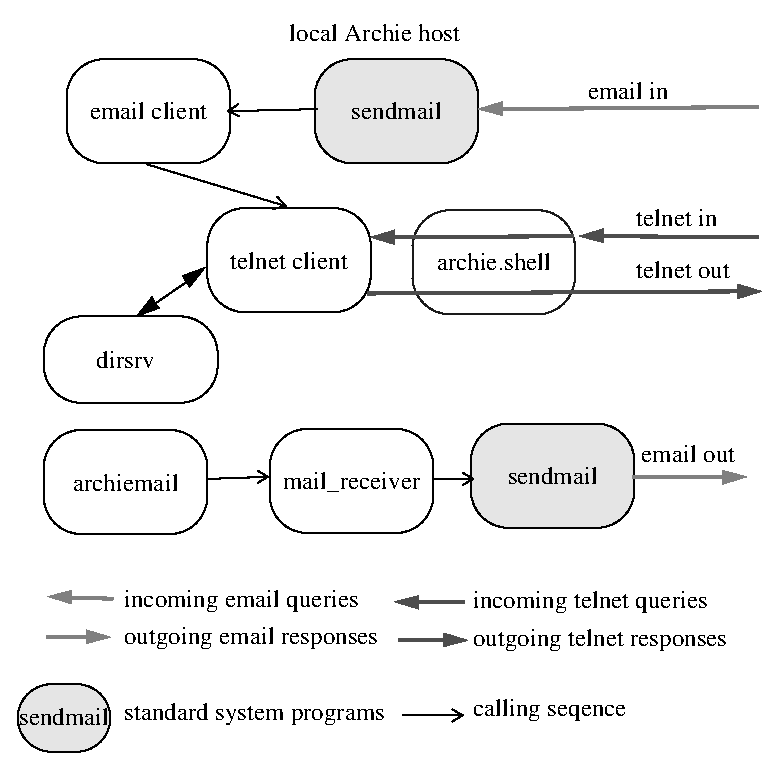
\epsfig{file=figs/telnet.eps,height=4in}
\end{center}
\caption{Archie system clients}
\label{fig:clients}
\end{figure}


\subsection{Client choices}

The telnet-client enables your user community to connect to an Archie server
and query the anonftp catalog through a standard telnet (remote login)
session. A user shell is provided and supports a query language to enable the
user to query the server. The email-client program enables users to send
electronic mail containing a series of commands to the Archie server which
will then be processed and returned in email to the user. You will have to
decide, as system administrator which of the supplied clients, if any you plan
to install. You should factor such things as

\begin{itemize}
\item Possible load on the system

\item Usefulness of the clients to your community

\item Administrative overhead
\end{itemize}


into your decision. The email and telnet clients can be run ``independently''
of one another in that you do not have to enable either one for the other one
to be made accessible.

\subsection{The  user system programs}

The following table describes the programs in the Archie user query
system. These programs can be found in the \Path{\archie/bin} directory.

\begin{tabular}{|l|p{5in}|}\hline

Program Name & Description \\ \hline \hline

telnet-client &

User interface via the telnet or rlogin protocols. The only program that
performs queries. Called by email-client to process queries. \\ \hline

email-client &

The user interface which processes incoming network email queries. \\ \hline

cgi-client &
The WWW interface that can be attached to your Web server to perform
queries. This will described in more details in section~\ref{sec:cgiclient} \\ \hline 

archie.shell &
Bourne shell script wrapper around the telnet-client which restricts the
number of simultaneous user telnet Archie sessions. (Optional). \\ \hline

archiemail &

``Front end'' to the Archie outgoing mail system. Used by the telnet-client
``mail'' command. Only used if the ``mail'' command or email-client are going
to be enabled. \\ \hline

mail\_receiver &

Does most of the work in sending mail to the user (generated by the ``mail''
command or from the email-client): parsing headers, compressing, encoding,
splitting and calling sendmail to mail the resulting data \\ \hline

split\_file &

Used to break large amounts of output into smaller pieces (if necessary),
since some mailers are only capable of dealing with messages of limited size.
\\ \hline
\end{tabular}


\subsection{The telnet client}

If you would like your user community to have access to the Archie system via
the standard telnet or rlogin programs, you should install the telnet client.

\subsubsection{Client privileges and security}

The installation phase (as described in ``Installing the basic Archie system''
on page~\pageref{chap:install}) will, in most cases, install the telnet client to operate as a
setuid (root) program. With these privileges, the client can change the
current

directory to the Archie home directory and call the chroot(2) system call to
make this the root of its own directory tree. This has the advantage of
reducing any unforeseen security problems when users use rlogin or telnet to
connect to the Archie server.



Whether the chroot call is made or not in the telnet client, the GNU less
program shipped with the Archie system has been modified to prevent the
examination of external files or execution of external processes. The modified
version of the sources for this program can be found in \Path{\archie/contrib.}




\alertbox{
The telnet client will relinquish its root status after it has performed this
chroot(2) system call, or exit if anything unusual occurs during the steps
leading up to (and including) the return from root status.

The telnet client will function even if it is not given permission to run with
root privileges.

For security reasons, on those platforms in which it is supported Bunyip
strongly recommends you install the telnet client to operate with root
privileges.}





If the telnet-client program is installed suid root and is running on a
platform which supports the chroot(2) security feature, copies of the system
files \Path{/etc/resolv.conf}, \Path{/etc/services}
(unless you are using NIS) and
\Path{/etc/termcap} must be placed in the \Path{\archie/etc} directory. This is because the
use of the chroot(2) system call will leave the original files inaccessible to
the Archie clients.





\subsubsection{Enabling the telnet mail feature}
\label{sec:telnetmail}

Most of the work of setting up the Archie client programs is done by the
installation script. However, you must first set up your system to accommodate
the new programs. This can be done as follows:

\begin{itemize}
\item
Create an archiemail entry in the /etc/services file (or the services
database, if you are running NIS) and in the \Path{/etc/services} file. For
example:

\param{archiemail 2709/tcp \#The Archie mail server}

\item
Create a corresponding entry in the /etc/inetd.conf file. For example:

\param{archiemail stream tcp nowait archie \Archie/bin/archiemail}

Don't forget to restart the inetd program (through the use of the UNIX kill
command, as described in ``The arserver program''on page~\pageref{sec:arserver}).


\item Create an alias, archie-errors, in the /etc/aliases file. This is where
errors generated by incorrect user mail addresses are sent, and is also the
Reply-To address in the mail responses sent to the user. To avoid dealing with
spurious email, you can set the alias to throw away incoming mail, by setting
the /etc/aliases entry to:

\param{archie-errors:/dev/null}

Remember to run, after these changes, the newaliases program or its NIS
equivalent (if you are using that system).

\item
Modify your sendmail configuration file. This is usually called sendmail.cf
and resides either in the \Path{/etc} or \Path{/usr/lib} directories. The
change that has to be made is to the T configuration lines. The default file
will look something like:



\param{\# Trusted users}

\param{Troot}

\param{Tdaemon} 

\param{Tuucp}

\noindent Now add the line:

\param{Tarchie}

This allows the Archie system to send mail with a ``Sender:'' of archie-errors
address. If this is not done, incorrectly addressed mail will bounce from the
remote mail receiver back to the Archie user, creating a mail loop which can
quickly fill your postmaster's mailbox.

After making this change you may need to ``compile'' your sendmail.cf file if
that is how your system is configured. Check to see if there is a file called
sendmail.fc in the same directory as the sendmail.cf file. If there is, the
run the following command:



\comm{sendmail -bz}


This will cause the sendmail configuration to be ``compiled'' (or ``frozen'').

\item
Modify the \Path{/etc/passwd} file for the archie user, with the full path for the
telnet-client program as the shell. For example:

\param{archie::23:1000:Archie User:<archie home>:<archie home>/bin/telnet-client}
\end{itemize}

\alertbox{
Note that, in this example, there is no password for the user archie. This is
normal for the operation of the most Archie installations. However, while you
are testing the system, you may wish to have a temporary password for this
account.}


Finally, check over the ``configure'' sections in the archiemail and
mail\_receiver scripts which reside in \Path{\archie/bin}. You should ensure that the
\Param{PATH} variable is correctly set to find the programs used by these
scripts. 



\subsubsection{Limiting the number of telnet sessions}
\label{sec:limit}

archie.shell is a shell script to limit the number of simultaneous connections
to the telnet-client.

\begin{itemize}
\item
Edit the archie.shell file to reflect the maximum number of simultaneous
sessions you want to allow, and the niceness level (see the UNIX manual entry
for nice(1)). The lines to be modified are clearly marked in the archie.shell
shell script.

\item
Edit the /etc/passwd file to change the archie user's shell from
telnet-client to archie.shell.

\item
A soft link between the telnet-client in \Path{\archie/bin} and -telnet-client
should exist from the default distribution. If it does not, run the following
command in that directory.

\comm{ln -s telnet-client -telnet-client}

\end{itemize}

\subsubsection{The .archierc file}

On start-up the telnet-client program reads a file called \Path{\archie/.archierc} if
it exists. The purpose of this file is to configure the program's behavior to
your particular needs. A number of variables can be set and commands executed
before the user prompt is generated. See the manual page archie\_clients(n) for
a complete explanation.

\subsubsection{Testing the telnet client}

Once the telnet-client program has been installed and configured, test it out
by performing a telnet session to the Archie host, and log in as
archie. Perform a ``find'' command to determine if everything is working
correctly.



\begin{itemize}
\item
The telnet client will not start on login:
\begin{itemize}
\item
Make sure the permissions on the file \Path{\archie/bin/telnet-client} are
correct. It should be executable by all, owned by root and run suid. That is
the ls(1) listing should look something like:

\param{---s--x--x 2 root 516096 Jul 16 02:22 telnet-client}
\end{itemize}


\item
The error message ``Can't resolve hostname (ardp)'' is displayed:

\begin{itemize}
\item
Check the telnet-client ``server'' variable (issue the command ``show
server''). It should be the valid name or IP address of an Archie host or in
many cases the name localhost if the telnet client and the dirsrv are running
on the same host.
\end{itemize}

\item
On start-up or after a command is issued an error is generated which says
``Timed out (ardp)'':

\begin{itemize}
\item
Check the telnet-client ``server'' variable (issue the command ``show
server''). It should be the valid name or IP address of an Archie host or in
many cases the name localhost if the telnet client and the dirsrv are running
on the same host.

\item
Make sure that the dirsrv process is running

\item
Check that the anonftp database has been initialized

\item
If using a remote (not local) Archie server host, it is possible that
network delays can cause this problem.
\end{itemize}
\end{itemize}


\subsection{The email client}
The email-client program allows users to access the Archie system via standard
Internet mail. It is in fact, just a specialized wrapper around the
telnet-client program which does the work of processing the incoming queries
(see Figure~\ref{fig:clients}). The requests from the email client are given
the lowest priority when queued on the Prospero server so as not to adversely
affect the operation of interactive clients.


The email-client can be used in one to two main ways, either ``interactively''
in which incoming email is processed as it is received, or ``batched'' in which
the incoming email is stored and processed later, usually at off-peak
times. In either case, to enable the email-client, first you need to enable
the telnet-client mail feature as described in section ``Enabling the telnet
mail feature'' on page~\pageref{sec:telnetmail}.

\subsubsection{``Interactive'' email requests}

For interactive email service add the following line to the /etc/aliases file.


\param{archie: ``| \Archie/bin/email-client''}



As usual, the newaliases program (or the NIS equivalent) will have to be run
in order for this change to take effect.

There are a number of options which can be provided to the email-client binary
including some to log incoming messages. See the archie\_clients manual page
for further details.



If your telnet-client binary is not installed as \Path{\archie/bin/telnet-client}
then you should use the ``-T'' option to tell the email client where the
telnet-client can be located.



\subsubsection{Batching email requests}
\label{sec:batch}

Email requests need not be processed directly as they are received on your
system. Instead, they can be batched and processed at a later (off-peak)
time. To do this change the standard entry in the /etc/aliases file to the
following:



\param{archie ``| <archie home>/bin/batch-email''}



By default, this will put each piece of mail in a separate file in
\Path{\archie/db/tmp}. You can override the temporary directory by using the -t
option to batch-email which will cause the email messages to be stored in an
alternate directory. You should make sure that this is a ``safe'' directory
whose contents will not be lost for example, on a system reboot.

You can then set your system to process the mail at a later time with the
process-email program.

\noindent For example, if you enter the line:



\param{0 1 * * * <archie home>/process-email}



into the crontab for archuser then each day at 01:00, the mail will be
processed. This also takes a -t option like batch-email to provide a different
temporary directory. process-email will process each piece of mail in
sequence.

\subsubsection{Testing the email client}

Test the email client by sending mail to \Param{archie@<your host name>}.  If
running as ``interactive'' email, a response should be generated in a number
of minutes. Note that this must be done from a machine other than the Archie
host due to the fact that on most systems, the sendmail program runs the user
daemon when mail is sent from off the local host, but as the user sending the
mail when run on the local host.



\alertbox{Email to the Archie server will not work from the Archie server host.}


\subsection{Auxiliary files}

The following files in \Path{\archie/etc} are used by the telnet-client and
email-client programs. They may be modified to reflect the local
configuration.


\begin{tabular}{|l|c|c|p{3.5in}|}\hline

Filename & \multicolumn{2}{c|}{Used By} & Description \\ \cline{2-3}
& telnet client & email client & \\ \hline \hline 

email.help & & x &
Response to a ``help'' command or an empty message. For any other form of more
specific help (e.g., ``help set''), the email-client returns the same
information provided by the telnet client. \\ \hline

manpage.ascii & x & x &
The pre-formatted version of the Archie manual page. \\ \hline

manpage.roff & x & x &
The troff(1) (or nroff(1)) version of the Archie manual page. \\ \hline

motd & x & x &
The ``message of the day'' that the email and telnet clients display to users at
the top of email messages or when they log in if set in dirsrv (See ``The
Message of the Day'' on page 52). \\ \hline

serverlist & x & x &
The list of servers given to the user in the ``servers'' command. \\ \hline

whatis & x & x &
The Archie whatis database. Entries (one per line) of short descriptions of
resources available on the network.
\\ \hline
\end{tabular}


\subsection{The Help system}
The Archie telnet and email client help system is rooted in the directory
\Path{\archie/help}. The system currently has full multi-lingual support. In order to
support languages other than the default supplied with the distribution, one
only need create a directory under \Path{\archie/help} with the name of that
language. For example a directory called francais would enable French language
support by allowing the users to type:



\param{archie> set help francais}



at the prompt in the telnet client or in the message body to the email
client. The files in the \Path{\archie/help/english} need then to be translated into
the new language. The files containing the actual data are called `=' and the
subdirectory names themselves provide the menu for that part of the help
system. See the manual page archie\_clients(n) for further details.


\subsection{Quoting in the clients}

For the email and telnet Archie clients, quoting in the command-line
interpreter is handled in much the same way as for the standard csh (see the
man page csh(1)). So, for example, the `.' can be treated as follows:



\param{LIST .il}

The `.' is treated as a regular expression

\param{LIST \\.il}

The `.' is quoted, and passed along (untouched) to the Archie search also if
you specify

\param{LIST il\$}

you will make sure that the host names returned end with the string ``il''.
For further details on regular expression consult the regexp(3) manual.





\section{Webindex catalog clients} 


This section takes a brief look at the WWW client. It provides access to both
webindex and anonftp catalogs.  Note that this section is still under
construction and any comment is very much welcomed. \new


\subsection{The cgi-client}
\label{sec:cgiclient}

The files are:

\begin{tabular}{ll}

cgi/html/archie.html      & Simple search form \\

cgi/html/archie-adv.html  & Advanced search form \\

cgi/html/archie-help.html & Help page \\

cgi/bin/archie.cgi & perl script called by the HTML forms \\ 

cgi/bin/cgi-client & binary called by the perl script \\

\end{tabular}



\subsubsection{Where to put them ?}

In order to provide a consistent way for accessing the Archie database,
we think that the urls should always be of the same format for
all public Archie server.

This format being

\path{http://archie.foo.bar/archie.html}

\path{http://archie.foo.bar/archie-adv.html}

\path{http://archie.foo.bar/archie-help.html}

We need to specify the \Path{.html} extension to ensure that all
WWW server will actually return the documents as  HTML documents. Otherwise,
some will presume that they are simply ascii.

\subsubsection{Configuration}

The configuration procedure is as follows:

\begin{enumerate}

\item Move the .html and .gif files to where your web pages are accessed.
\item Move (or link) ``archie.cgi'' to the cgi-bin directory of your web server.
\item
Edit the html files ``archie.html'' and ``archie-adv.html'' to reflect
the appropriate path of the cgi script ``archie.cgi'' after you have placed
it in the right path.

\item 
Edit the file ``archie.cgi'' and configure the first few lines as indicated
in the file.

\item Make sure that the UID for the ``cgi-client'' binary is set.


\item
Test the forms and if you don't like the format of the output, take a
look at the ``archie.cgi'' perl script and edit the output variables to your
convenience.
\end{enumerate}


\subsubsection{How does it work}

The ``archie.cgi'' perl script receives a query (from the archie*.html forms)
and calls up ``cgi-client''. The cgi-client binary processes the request and
sends the results to the perl script in plain record-template format.
``archie.cgi'' reads the results, reformats the output into HTML and then
sends the new output to the web server.



\subsubsection{How to reformat the output}

``archie.cgi'' is the perl script you need to modify.  The second segment
after the configuration part holds the variables that are sent back to the
Web server.  Configure any variable to your needs.
  

\subsubsection{Where is the information logged}

``cgi-client'' logs queries, the number of hits and any error messages to a
file in the log file \Path{\archie/logs/query.log}




%
% Copyright (c) 1996 Bunyip Information Systems Inc.
% All rights reserved
%
% Archie 3.5
% August 1996
%
% dirsrv.tex
%


\Chapter{The Archie/Prospero server (dirsrv)}


The basic Archie system is primarily concerned with the location, retrieval
and collation of data on the network and does not explicitly define a method
to serve this information to the end-user. However, a close relationship
between Archie and the Prospero Virtual System exists: all of the most popular
freely-available Archie clients as well as those provided by Bunyip use the
Prospero protocol to communicate with a modified Prospero server. This server
allows users to search and access the various Archie catalogs.



The Archie system includes a Prospero server, modified from the
freely-available version, to accommodate many of the new features that Archie
offers. The directory \Path{\archie/pfs/bin} contains the complete range of
pre-compiled Prospero binaries that are supplied for your convenience.

The Prospero binaries that are supplied have been modified based on the
directory structure in the Archie distribution and are rooted in the
\Path{\archie/pfs} directory.

If this structure is changed, the system will need to be recompiled. Please
check the Prospero configuration files to make sure that they are correct for
your installation.



\alertbox{The modified Prospero server retains the full functionality of the
basic Prospero system and can be used as such. Please see the Prospero
documentation or send mail to info-prospero@prospero.isi.edu for more
information.}





\section{Configuring the server}

The Archie/Prospero server needs to be configured before it is started.




\subsection{Configuring dirsrv for the catalogs}

Before you start the server, you may need to modify the dirsrv configuration
file, \archie/etc/catalogs.cf. This file tells dirsrv the catalogs to serve to
the outside world and where they reside. It has the following format:

\param{<catalog name> <type> <access method> <location>}


\param{<catalog name>} The name of the catalog. Now anonftp !

\param{<type>} The type of catalog, For the moment this is always archie.

\param{<access method>} The way this catalog is accessed. See text below.

\param{<location>} Pathname, relative to \archie/db of where this catalog resides.

For example, here is the default catalogs.cf file that comes with the Archie
system distribution.


\param{\#}

\param{\#This is a comment}

\param{\#database type access method location}

\param{\# name}

\param{anonftp archie anonftp anonftp\_db}




Note that comments can be placed in the file with the use of a ``\#''
character. The comment continues from that character to the end of the current
line. Any configuration line may be continued on to the next line with the use
of a ``\\'' character at the end of the line to be continued.

%In this example, the system serves two catalogs, anonftp and gopherindex both
%having a type of archie. This means that these catalogs are specific to the
%Archie system which also defines their access methods, anonftp and gopherindex
%respectively. The last field specifies the path of the data files for these
%catalogs relative to the \Path{\archie/db} directory. Thus, the data files for the
%anonftp catalog can be found in \Path{\archie/db/anonftp\_db} while those for the
%gopherindex catalog can be found in \Path{\archie/db/webindexrindex\_db}. As the
%system evolves, new types and access methods will be defined to allow the
%server to access other kinds of catalogs.



\subsection{Starting the server}

\alertbox{You will require root access to perform the following operations.}


The following line may be added to the /etc/services file (or to the
appropriate NIS file, if it is running on your host). However, the server will
operate without this line being present.



\param{dirsrv 1525/udp}



To allow the Prospero server to start whenever the Archie server machine is
rebooted, the following command should be added to the end of the
/etc/rc.local file on the Archie server host.

\comm{<archie home>/pfs/bin/pstart}

where \Param{<archie home>} is the full path of Archie home directory.

You may also start the Prospero server manually by issuing the pstart command
from the command line. If a version of the program is already running, an
error message will be displayed and the new version will not start.

The pstart program should be set to have the Archie group as its group. This
can be achieved as follows:

\comm{chmod g+s pstart}

This will normally be done by make when initially installing the system.

The pstart process is responsible for starting the program, dirsrv which
actually performs the queries. This program must not be renamed, or else it
will not be able restart automatically in case of failure.

\alertbox{dirsrv makes extensive use of the files in \Path{\archie/db}. If you plan
to do extensive work on these files (such as rebuilding the databases there),
make sure that dirsrv is terminated and restarted after the work is 
complete. Failure to do so may cause the program to fail or operate
unpredictably.}



\alertbox{The Archie/Prospero server dirsrv in normal operation writes all log
messages to the file \Path{/pfs/pfs.log}}



It is possible in theory simultaneous heavy update and query loads will cause
the dirsrv program to fail. In general, it's best to plan catalog updates for
off-peak query hours.




\section{The dirsrv log files}

The dirsrv program writes its logging information to the file
\Path{/pfs/pfs.log}. This file contains information about the general operation of
the server (startup times, errors encountered etc.) and the user queries
processed. Lines containing the string ARCHIE/MATCH signify searches in the
anonftp catalog. See the manual sections in the catalog for a detailed
description of the syntax of these log entries.



\alertbox{\begin{center}IMPORTANT\end{center}
Information contained in the dirsrv log file must be considered confidential
and should not, under any circumstances, be released without first removing
any information which may identify individual users or hosts from which the
queries originated.}



\section{The Message of the day}

The administrator can set a ``Message Of The Day'' on the Prospero server via
the use of the padmin command found in the \Path{\archie/pfs/bin} directory. This
message will be available to all remote Archie (Prospero) clients and is
normally displayed by the telnet and email clients for the anonftp catalog
supplied with the Archie distribution. You can either prepare a file
beforehand containing the message that you want installed or you can type it
on the command line. You then issue the command as the superuser (root):


\comm{padmin -set MOTD < messagefile}



If you do not redirect the input the program will prompt for the message on
the command line and read it in from stdin. You may wish to put this line in
your \Path{/etc/rc.local} file as the MOTD is only set through the padmin
command will not be ``''remembered'' between host reboots or crashes.


\begin{itemize}

\item The Archie/Prospero server will not start: \NOTE

\begin{itemize}
\item 
Make sure the pstart program has setgid permissions and that it is owned by
the archie group.
\end{itemize}

\item dirsrv complains ``cannot bind to socket'':

\begin{itemize}
\item 
There is another dirsrv process already running.
\end{itemize}

\item
the server will not respond to queries from Archie clients

\begin{itemize}
\item 
Check the log file for possible error messages explaining the problem.

\item
Check to make sure that the \Path{\archie/etc/catalogs.cf} file is correctly
configured.

\item
Make sure that the permissions on all files in the \Path{\archie/db} directories
are correct.

\item
Check to see if the server is running under heavy server load. If it is, the
query may just be taking a long time to execute. This can be done by
monitoring the log file and checking the ongoing use of the system.

\item
 Make sure that the catalogs that you wish to access have been
initialized. The Archie/Prospero server requires that the catalog desired has
been initialized before any queries can be processed. See the section on the
particular catalog for more details.
\end{itemize}
\end{itemize}


\section{The Log file}

The dirsrv process logs client requests to the file \Path{/pfs/pfs.log}. Lines
containing the string ARCHIE/MATCH signify searches of the anonftp catalog,
while entries with ARCHIE/HOST contain queries related to the telnet-client
list command. The syntax of the two entries are described below. Note that the
`/' character acts as a separator in the Prospero system.



\subsection{The MATCH request}

A typical anonftp catalog search query is (this is split here across two lines
for readability).


\begin{center}
\texttt{4-May-94 19:08:03 127.0.0.1(root)[ggB(P53.3Mar94)] - L
ARCHIE/MATCH(15,100,100,0,=)/public\_access *}
\end{center}

\begin{center}
\begin{tabular}{|l|p{4in}|} \hline
Field Contents & Description \\ \hline\hline

4-May-94 & Date of query \\ \hline

19:08:03 & Time of query (local) \\ \hline

127.0.0.1 & 
IP address of host where query originated. Note that for the telnet and email
anonftp catalog clients the will ususally be 127.0.0.1 (localhost). \\ \hline

(root) & 
Name of user sending the query. For the telnet and email clients this will
normally be archie. If the email is being run in ``interactive'' (not batched)
mode, this user will be daemon. \\ \hline

[ggB(P53.3Mar94)] & 
Client ID. All Prospero-based clients are allocated by the Prospero group
(info-prospero@prospero.isi.edu) a unqiue identifier. This identifier is
changed with each new version of the client. \\ \hline

ARCHIE & 
Specifies to Prospero that this query is intended for the Archie subsystem. \\ \hline

MATCH & Search of the anonftp catalog \\ \hline

(15,100,100,0,=) & 
Paramters to the search. The first 3 values set the maxhits, maxmatch, and
max\_hitspm variables respectively. The 4th value (``0'') is the ``offset'',
currently unused. The final charater specifies the type of search to be
performed. Possible values and meanings are: 

\begin{tabbing}
= \= exact \\ 
R \> regex \\
r \> exact\_regex \\
X \> string-only regex \\
x \> string-only exact\_regex \\
C \> subcase \\
c \> exact\_subcase \\
K \> string-only subcase \\
k \> string-only exact\_subcase \\
S \> sub \\
s \> exact\_sub \\
Z \> string-only sub \\
z \> string-only exact\_sub \\
n \> string-only exact \\
\end{tabbing}
\\ \hline

``public\_access'' & String to be searched for \\ \hline
\end{tabular}
\end{center}


\subsection{The HOST request}

The HOST Prospero request is used to perform both the telnet-client list as
well as the ``directory expansion'' feature found on some Archie clients
(notably xarchie). The function performed is determined by the form of the
final argument: if it is a regular expression the list function is carried
out, otherwise the argument is taken as the host and pathname of a directory
to be expanded. HOST commands have the following syntax:



\begin{center} \texttt{2-May-94 01:32:23 132.206.35.4(suzie)[B42E] - L
ARCHIE/HOST/sequoia.ccsd.uts.edu.au/pub}
\end{center}

\begin{center}
\begin{tabular}{|l|p{4in}|} \hline
Field Contents & Description \\ \hline\hline

2-May-94 & Date of query \\ \hline

01:32:23 & Time of query (local) \\ \hline

132.206.35.4 &
IP address of host where query originated. Note that for the telnet and email
anonftp catalog clients the will ususally be 127.0.0.1 (localhost). \\ \hline

(suzie) & Name of user sending the query. \\ \hline

[B42E] & Client ID. \\ \hline

ARCHIE & 
Specifies to Prospero that this query is intended for the Archie subsystem. \\ \hline

HOST & list or ``directory expansion''. \\ \hline

sequoia.ccsd.uts.edu.au & 
Hostname to be expanded. If this value contains regular expression characters
(such as ``*'' or `]') then the names of all sites matching that expression are
returned (the list command). \\ \hline

pub/xntp &
Directory pathname to be expanded. That is all files and subdirectories
contained within the given directory (if it exsits) will be returned. \\
\hline
\end{tabular}
\end{center}



%
% Copyright (c) 1996 Bunyip Information Systems Inc.
% All rights reserved
%
% Archie 3.5
% August 1996
%
% faq.tex
%


\chapter{Frequently Asked Questions}


This chapter contains a list of Frequently Asked Questions which have been
compiled during the operation of Archie over the past several years. It is
hoped that it can serve as a quick reference to some of the more common
problems associated with running an Archie server.

We hope to regularly add new questions and answers to this chapter and
make it available as a stand-alone postscript document in your
account on ftp.bunyip.com.

\section{General}


\Question{We have DNS. Why does Archie need to store the IP address of a
particular host?} 

\Answer{
Archie uses IP addresses internally to provide a form of ``unique identifier''
within the host databases. The Archie system tries to avoid having the same
physical host listed in the database under different names (which hosts can
have through CNAME records). One can see why when one realizes that if Archie
didn't try to do this, then the same host could potentially be indexed several
times for each one of its several names. As a result, Archie tries to use the
IP address as a kind of ``unique identifier'' for the host. The system stores
the primary host name (the DNS A record) as well as the primary IP address for
that host. In most cases, this IP address changes infrequently and serves the
purpose. In the case that the host has multiple IP addresses (interfaces) DNS
will normally return a ``primary'' address: this tends to be the first PTR
record under DNS. You may notice that in the site files for the anonftp and
webindex databases, the IP address is used as the name for the site
file. The system is designed to detect when a primary IP address has changed
and modify its internal information.


In addition to the internal uses of the IP address, some users, particularly
those on the MILNET don't have access to the DNS. As a result, Fully Qualified
Domain Names can't be used and the IP addresses are their only route to the
archives of the world.
}



\Question{Can I mount the Archie temporary directory (\archie/db/tmp) on another
partition?
}

\Question{Can I mount the Archie catalogs (\archie/db/*) on another partition?
}

\NOTE

\Answer{Yes and no... The only restriction at this point is to have
\Path{db/tmp} and \Path{etc} in the same partition. If a database, for example
\Path{db/anonftp\_db}, resides in a different partition, the files will be
copied instead of being moved, resulting in slower execution.}


\Question{The hostname on my Archie server doesn't contain the fully qualified domain
name. When I try to collect data from anonymous FTP sites that require a
password with a FQDN (like foo@bar.com instead of foo@bar) the process
fails. How do I get the system to send a fully qualified domain name?
}

\Question{The primary name of my Archie server host is ``foo.bar.com'', but I want the
Archie system to use the alias ``archie.bar.com'' (CNAME record) when it
contacts remote sites and for the ``Source:'' line in the host\_manage program
display. Can this be done?
}

\Answer{
Yes, if you create a file called \archie/etc/archie.hostname which just
contains the hostname that you would like Archie to call itself then
everything will work the way you would like. Note that the name of that file
is exactly that ``archie.hostname''. ``hostname'' is not a variable to be replaced
by some other name.
}



\section{Clients}

\Question{Even with the autologout feature, some sessions on the telnet-client still
seem to hang around even though they have been idle for a long time. Why?
}

\Answer{
The problem usually occurs when users suspend the telnet-client in the process of sending data to the tty (remote connection). The client will try to perform the autologout, but can get suspended trying to close the connection at the other end. We are looking into possible solutions.
}



\Question{How do I tell how many people are using the system?
}

\Answer{
The question here usually is, ``how many queries am I getting?''. The easiest
way is to look in the file \archie/pfs/pfs.log and count the lines that have
ARCHIE in them (grep -c will do this for you). If you want to get fancy you
can separate the lines by date (each line is date and timestamped) to get a
count on a per-day basis. You can count the number of people using the telnet
client by using the last(1) command (``last Archie'' should do it) and you can
count the number of queries and users on the email interface by enabling the
logging (-u and -l or -L) and counting the lines in there.
}


\Question{How do I restrict the number of concurrent telnet sessions?
}

\Answer{
Look in the chapter ``Setting up the anonftp catalog clients'' in the section
``Limiting the number of telnet sessions'' on page~\pageref{sec:limit}.
This will explain what you need to know.
}



\Question{Why does mail returned from the Archie email interface say that it
comes from ``archie-errors''?
}

\Answer{
This is a historical ``accident'' with no real meaning. The problem addressed is
that if mail came back ``From: archie'' and it bounced (for whatever reason)
then the bounced mail would go right back to the Archie server which would
then try to interpret it. In most cases the email interface would generate a
help message which would then probably bounce again etc., etc. As a result,
mail headers get rewritten so that they bounce to a ``bit bucket'' and get lost
forever. We do not suggest that you point the alias of ``archie-errors'' at a
file or a person.... it or they will probably get a lot of bounced mail that
was generated because some user made a typo. The name ``archie-errors'' can be
changed to anything you like however but it will require a slight modification
to the system. If you are interested send mail to the Archie contact address
here at Bunyip and we'll tell you how to do it.
}

\Question{One of our users is connected to us on a slow (9600 baud) SLIP link and when
using an Archie client the whole link becomes unusable. Is there a problem
with Archie on slow links?
}

\Archie{
Yes. Archie uses the Prospero system as its transport mechanism. Prospero is a
UDP based protocol so when errors occur and packets go missing it is the
responsibility of the dirsrv process to perform the retransmissions. On slow
links the time allocated for the client to acknowledge receipt of the server
packets may expire even though the client has received the packet. As a result
the server and client go into a competition to transmit each other packets and
this can bring the link to a halt. We know about this and is working on a
solution to the problem.
}

\Question{Instead of having the email-client run every time a piece of mail to the Archie address arrives, can I batch the mail and have it processed at off-peak times?
}

\Answer{
Yes, you can. The program \archie/bin/batch-email will allow you to do
this. See the section ``Batching email requests'' on page~\pageref{sec:batch} for an explanation.
}


\section{The Host Database}

\Question{How do I change the primary name of a host in the Host Database?
}


\Answer{
Because the Archie system ``keys'' on the primary hostname of a host, changing
its value requires a deletion of the host from the database followed by a
re-insertion with the new name. See ``Deleting a Data Host'' on page~\pageref{sec:delhost}.
}



\Question{How do I add a site to the Host Databases so that I can index that site?
}

\Answer{
Details for this procedure can be found in the section ``Adding individual Data Hosts'' on page~\pageref{sec:addhost} of this manual.
}

\Question{How do I completely delete a site from my Host Database?
}

\Answer{
You can either use the host\_manage program. See the manual
pages for further details.
}

\section{Parsing}

\Question{Why does the error line number reported by the parser not correspond to the
actual line number that caused the error?
}

\Answer{
This is a bug in the system. Basically, the number of the line reported is
counted from the start of the listing. However, the Archie header adds 8-10
additional lines at the top of the file, causing the mis-count. The actual
line causing the error is in fact the number of lines in the header plus the
line number reported by the parser. This will be fixed in a patch, soon to be
released.
}

\section{Data Exchange}

\Question{I am exchanging data with another Archie server and even though things seem to
be working OK (I run arexchange with the -v option and data is being
transferred), I don't get any data files in the \archie/db/tmp
directory. What's happening?
}

\Answer{
The problem results from a combination of things. First, the site with which
you are exchanging data has a set of catalog entries which have been
deleted. In order to allow this information to be propagated to sites like
yourself, the system holds on to these records for a while, until the Archie
administrator at the remote site physically deletes the information from his
or her Host Database (with the purge\_hostdb command). When this has not been
done in a long time (or a lot of catalog entries have been deleted recently),
these records will be transmitted to you so that your Archie system can delete
those entries itself. However, your system is smart enough to recognize that
if you didn't have those entries in the first place there is no need to
download a ``deletion'' record for them. Therefore the data that you see being
exchanged is really a set of deletion records but since you don't have those
entries anyway, your system is ignoring them. The problem comes when you are
asking for 50 entries at a time from the remote system and they have more than
50 deleted entries.... you end up with nothing. The solution to the problem is
to contact the remote Archie administrator and ask them to run the
purge\_hostdb command and do some garbage collection.
}

\Question{When I try to do an exchange with a remote Archie server I get a message
saying ``Network command not terminated with a CR''. What is the problem?  }

\Question{When trying to connect to my local arserver program with arretrieve, I get the message, ``Read EOF from network connection''. What's up?
}

\Answer{
The arserver process to which you are talking not starting correctly. For
example, if arserver sees an option in its command line in
\Path{/etc/inetd.conf} which it does not understand, it writes the error
message to stdout. Now inetd connects stdout of the processes it runs to the
network connection and so you are seeing whatever errors arserver is
printing. Note that this problem almost only occurs on start-up of the remote
server before it has time to read its options and open its log file, otherwise
it would write the errors to its own log file. The solution is to contact the
Archie admin of the remote site and ask them to look into the problem. If it
is happening to you with the arretrieve program then the same thing
applies. Check the information on the command line to arserver in
\Path{/etc/inetd.conf} and make sure it is OK. You can also check the Archie
log and search for ``arserver'' and see if wrote any errors there.
}


\section{Prospero and dirsrv}
\Question{If I have made changes to the databases, do I have to restart the dirsrv
process?
}

\Answer{
If you have just made normal, everyday changes to the database then you don't
have to restart the dirsrv process. However, if you have added an entire
catalog (for example, the anonftp catalog) then you will have to kill and
restart dirsrv. For efficiency, dirsrv keeps certain files open all the time
(rather than opening and closing them on every query). If you delete the
catalog, dirsrv won't know about the new entries and will try to reconcile the
files it has open with the new ones, usually killing the process. You can
prevent this senseless death by killing and restart the process yourself.
}


\Question{I have noticed the dirsrv process crashing, what's wrong?
}

\Answer{
The dirsrv process can crash for one of two reasons: (a) the database is
corrupt or (b) the database is being updated at the time of the crash. Both
are due to ``incorrect'' pointers in the database the first possibly being
permanent the second being transitory. Consistency checking is kept to a
minimum in order to speed up the searching process.

db\_check attempt to determine if the various
elements in the catalog are consistent. Unfortunately, due to the complexity
of the catalog structure it is not always obvious how the errors reported by
dirsrv are connected to those listed by db\_check. Minor inconsistencies
given by WARNING messages from db\_check are informational in nature and
don't affect operations. ERROR messages are more serious. db\_check
should be run while the catalog is quiescent (not being updated) for a real
reading of the current status. If it reports errors, I would advise another
update cycle be run and the catalog checked again before worrying about
rebuilding it. However, as a rule if pages of errors are reported it is likely
that the catalog has been corrupted.
}

\section{Catalogs}

\Question{How do I tell if the one of the catalogs is corrupted?
}

\Answer{
Well, there are a number of ways. First, check the log file for the word
``corrupt''. The dirsrv process does some minor checks to make sure
everything is okay during its normal operation. (Note that these checks are not very complete as they would slow down the performance of the server and we'd like it as fast as possible). Secondly, if the update cycle fails with programs terminating abnormally, then you could have a problem. For the anonftp catalog (and some others) there is a program called ``check\_<catname>'' where <catname> is the name of a catalog. So, for example, there is a program called ``check\_anonftp''. This program will try to do some comprehensive consistency checking and report what it has found. It may report some messages as ``WARNING'' which usually means that something is a bit out of order, but nothing serious. If you get ``ERROR'' messages however, you probably have a corrupt catalog (if the program crashes you definitely have a corrupt catalog).
}


\Question{How do I fix a corrupt anonftp or webindex catalog?
}

\Answer{
Try running the program fix\_start\_db if the program db\_check says so.
If a single site is corrupt, by re-inserting it, the problem should go away.
}


\Question{What causes the anonftp or webindex catalogs to become to become corrupt?
}


\Answer{
The catalogs can become corrupted in two main ways:

\begin{itemize}
\item
The host crashes or is rebooted during the update phase of the cycle when the
catalogs are being modified. Therefore it is important therefore that the
system not be intentionally rebooted when an update is occurring. Of course,
host crashes are usually unintentional and can't be prevented.

\item The insert\_anonftp or insert\_webindex program terminates abnormally
during an update. This is rare, but can happen as a result of the system core
memory being exhausted. The insertion routines are written in such a way that
once modifications to the catalog files begins, very little memory is required
from the system. However, if the host has no more available memory, even a
little will be refused.
\end{itemize}

In either case, you should perform the routine appropriate for the particular
catalog to see if it has been corrupted. If it has the restoration procedure
will have to be invoked. In either case the anonftp or
(webindex) file will be left around in the \archie/db/locks directory
to mark this fact. (This will be reported if you have the system set up to
mail you status reports).  }


\Question{Why the database get larger and larger over time?
}

\Answer{
Well, for one thing, there are more and more machines on the network. However,
this is not the only reason. The other major one is that due to the way that
Archie keeps the strings in the database, ``dead'' information can collect over
time. For example, one anonymous site contains a filename like ``furglesnort'',
it is indexed by the anonftp catalog and then the site removes the
file. However, the anonftp catalog will keep the ``furglesnort'' string in the
database (marked inactive) for the rest of time. As a result, such strings
build up in the catalog never to be used. While it would be possible to
``garbage collect'' in the catalog, the structure would require that enough
space exist to build a copy of the catalog during the process. The catalog for
anonftp is on the order of 500 Mb now so this is not really a viable
option. We recommend that the database be rebuilt ever six months or so to
remove the dead records.
}

\section{Database}
\new


\Question{Why does the file Stridx.Lock stay around?}

\Answer{
The file is used to perform locking through the lock(2) and flock(2)
mechanisms for building the index file.
The presence of the file does not indicate that the index is locked.
}

%
% Appendix
%

%
% Copyright (c) 1996 Bunyip Information Systems Inc.
% All rights reserved
%
% Archie 3.5
% August 1996
%
% appendix.tex
%


\begin{appendix}



\chapter{Header record}
\label{app:header}


The following header record fields are currently used by the Archie system:


\setlongtables
\begin{longtable}[!]{lp{4.5in}}
Field Name & Function \\ \\  \hline \\
\endhead
\endfoot

primary\_hostname & 
The primary hostname of the site to which the data belongs. These names are
used internally by the Archie system
 \\

preferred\_hostname &
The name under which users see this site listed. It will be a valid Domain
Name System canonical name (CNAME) for that site if one has been set \\

generated\_by & 
The component of the Archie system which has generated this header. Valid
values are: 
\begin{TTentry}{retrieve}
\item[parser] Output from the parse phase
\item[retrieve] Output from the data acquisition phase
\item[server] Generated by the data retrieval phase
\item[admin] Generated by an administrative procedure
\item[control] Generated by the controlling routines (usually after an error)
\item[insert] Generated by normal update routines (seldom seen)
\end{TTentry} \\

source\_archie\_hostname &
The name of the Archie server responsible for monitoring information at this
Data Host \\

primary\_ipaddr & 
The primary IP address of the Data Host used internally by the Archie system \\

access\_methods &
The name of the Archie catalog to which this data belongs. E.g., anonftp (for
anonymous ftp listings), webindex (for WWW pages) etc .. \\

access\_command &
The catalog-specific sequence of parameters used during the Data Acquisition
phase to perform the acquisition of the raw data from the Data Host. \\

os\_type & 
The operating system type of the Data Host. \\

timezone & 
The timezone of the Data Host. \\

retrieve\_time &
The time of data acquisition from the data host. This is written as
YYYYMMDDHHMMSS (year, month, day, hour, minute, second) and is always in UTC
(GMT). \\

parse\_time &
The time the data was parsed. Written in the same format as the retrieve\_time
field. \\

update\_time &
The time the data was updated. Written in the same format as the retrieve\_time
field. \\

no\_recs & 
The number of ``records'' in this data. For example, the value for a file
listing would be the number of files in the listing. This field is not used by
all catalogs. \\

current\_status &
Lists the current status of the data host. This can be:

\begin{TTentry}{del\_by\_archie}
\item[active]     available to be queried and inspected
\item[inactive]   temporarily disabled by the system
\item[del\_by\_archie]   scheduled to be deleted. Usually means that the data
in the system is out of date
\item[del\_by\_admin] scheduled to be deleted by the local administrator
\item[disabled] deactivated by the local Archie administrator
\item[not\_supported] catalog type is not supported at this data host
\end{TTentry} \\

update\_status & 
One of fail or succeed. Used internally by the system to determine result of
the previous phase of the update. \\

prospero\_host &
One of yes or no describing if the Prospero system is in operation at that
site. \\

data\_name & 
Name of individual data in current file. \\
\end{longtable}





\end{appendix}


\end{document}
